% ===========================================================================
% Standalone wrapper so that methods.tex compiles on its own.
%
%   pdflatex main            (run twice, so that \eqref and \ref resolve)
%
% To drop the Methods section into a host manuscript instead, copy the macro
% definitions from preamble.tex into that manuscript's preamble and
% % ===========================================================================
% Methods section. Numbering is automatic and sequential; every cross-reference
% uses \eqref, so inserting or removing an equation renumbers the section
% consistently without hand-editing.
% ===========================================================================
\section{Methods}
\label{sec:methods}

\subsection{Overview of the modelling framework}
\label{sec:overview}

Autologous CAR-T therapy couples a manufacturing supply chain to a
deteriorating patient. Each therapy is patient-specific and
non-substitutable: the cells collected from a patient can be manufactured
only for that patient, so a delay in the network is not a delay in inventory
but a delay in treatment, borne by a patient whose probability of surviving to
infusion is falling. Conventional supply-chain models treat time through a
deadline---a maximum admissible turnaround---which is a binary and tier-blind
representation of a hazard that is in fact continuous and tier-specific. The
framework developed here replaces the deadline with an explicit survival
model, and in doing so makes clinical prioritisation an \emph{output} of the
optimisation rather than an input rule.

The framework has two layers, solved in sequence (Figure~\ref{fig:framework}).

The \textbf{strategic layer} (\S\ref{sec:strategic}) is a mixed-integer linear
program that extends the patient-centric supply-chain design platform of
Triantafyllou et~al.\ \cite{triantafyllou2022} in two ways. First, it
introduces a genuine manufacturing
queue: the start of manufacturing becomes a decision variable constrained by
material arrival and by concurrent facility capacity, so a job may be
\emph{held}. Second, it prices that hold clinically, through a patient-level
survival function embedded exactly in the objective. The layer decides
facility locations, patient--facility assignment, transport modes, and a
nominal schedule.

The \textbf{operational layer} (\S\ref{sec:epoch}--\S\ref{sec:sim}) freezes the
strategic decisions and asks the question the deterministic model cannot: what
happens when manufacturing actually fails? A daily discrete-event simulation
advances the clock over the planning horizon, realises manufacturing yield as
a Bernoulli outcome at release testing, evolves each patient's survival with
the accumulated wait, and at every epoch at which a manufacturing slot frees
calls a small look-ahead optimisation that decides who starts next on the
\emph{observed} state. Manufacturing failure triggers a re-collection recourse
gated on projected survival.

This separation is deliberate and reflects the decision horizons of the real
system: facilities and contracts are committed once, over years; sequencing
decisions are made daily, under information that did not exist when the
network was designed. It also yields a clean identification strategy. Because
the network is frozen and shared across every policy we compare, and because
manufacturing failures are generated by common random numbers keyed to the
patient and attempt rather than to call order (\S\ref{sec:design}), any
difference in outcome between two policies is attributable to sequencing
alone---not to a different network, a different cost structure, or a luckier
draw.

\begin{figure}[htbp]
  \centering
  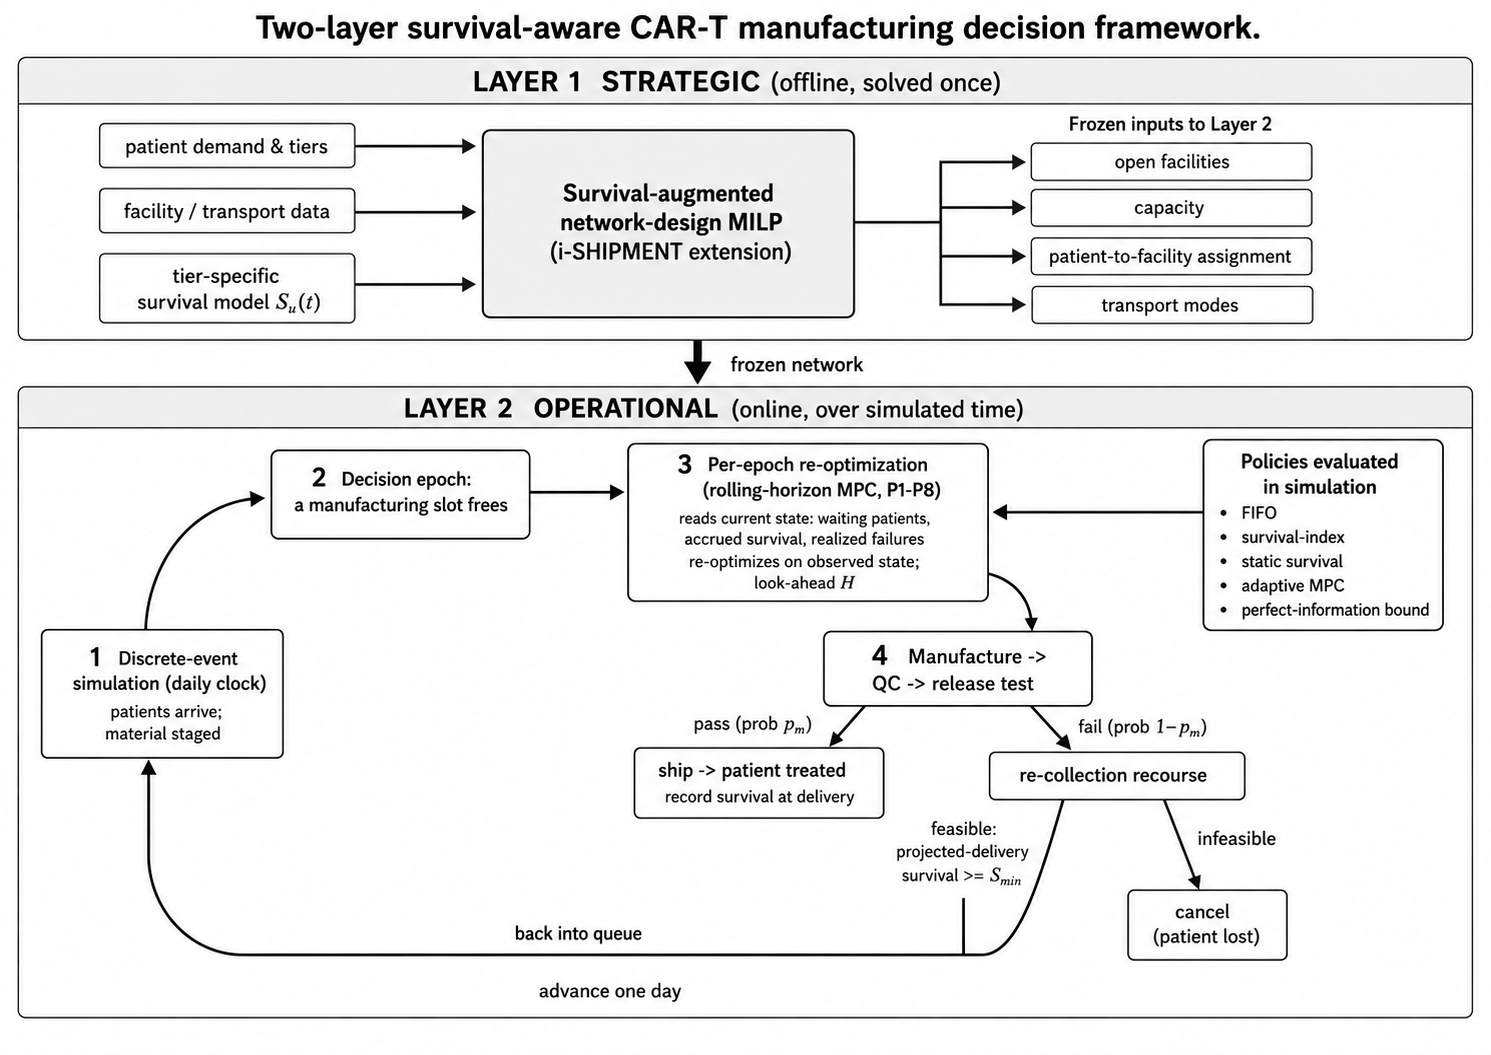
\includegraphics[width=\textwidth]{figures/Framework.png}
  \caption{\textbf{Two-layer survival-aware scheduling framework.} The
  strategic layer is solved once and fixes the network---open facilities,
  capacity, patient--facility assignment and transport modes. The operational
  layer executes on that frozen network: a daily discrete-event simulation
  realises manufacturing yield, and at each epoch at which a slot frees the
  per-epoch problem re-optimises on the observed state over a look-ahead
  window $H$, implementing only the immediate start. A failed batch returns
  its patient to the queue subject to the re-collection gate, or is
  cancelled. All five policies enter at the per-epoch decision point and
  differ only there.}
  \label{fig:framework}
\end{figure}

\subsection{Notation}
\label{sec:notation}

Sets: patients $p \in P$ with risk tier $u(p) \in \{H, M, L\}$; manufacturing
sites $m \in M$; leukapheresis sites $c \in C$; hospitals $h \in H$; transport
modes $j \in J$; periods $t \in T = \{1, \dots, 130\}$; and $\Theta \subset C
\times H$ the set of co-located leukapheresis--hospital pairs.

Parameters retained from the base model: capital and variable facility cost
$\CIM_m$, $\CVM_m$; concurrent capacity $\FCAP_m$; unit transport costs
$\Uone_{cmj}$, $\Uthree_{mhj}$; transport times $\TTone_j$, $\TTthree_j$;
stage durations $\TLS$, $\TMFE$, $\TQC$; per-therapy material and
release-testing costs $\Cmat$, $\CQC$; the arrival incidence $\INC_{pct}$; the
flow bounds $\FMIN$, $\FMAX$; and the maximum turnaround $\ND$.

Parameters introduced here: the tier reference mortality $w_u$ and the induced
hazard $\HR_u$; the survival scale $\eta$ and shape $\gamma$, and sensitivity
$\kappa$; the per-tier value of life $\alphau$; the manufacturing yield
$p_m$; the look-ahead horizon $H$; the re-collection floor $\Smin$; the
maximum number of remakes $\Krem$; and the re-leukapheresis cost $\creleuk$.

Decision variables retained: facility opening $\Eone_m \in \{0,1\}$; link
activation $\Xone_{cm}, \Xtwo_{mh} \in \{0,1\}$; patient routing
$\Yone_{pcmjt}, \Ytwo_{pmhjt} \in \{0,1\}$; the material flow variables
$\LSA$, $\LSR$, $\MSO$, $\OUTC$, $\OUTM$, $\INM$, $\DURV$, $\FTD$, $\INH$; and
the timing variables $\STT_p$, $\CTT_p$, $\TRT_p$. Variables introduced here:
the survival rate $S_p \in [0,1]$; the queue delay $\HOLD_p \ge 0$; the
material arrival $A_{pmt}$; and the survival indicators $\delta_{p,d} \in
\{0,1\}$.

\subsection{Strategic layer: survival-aware network and queue design}
\label{sec:strategic}

\subsubsection{Relationship to the base model}
\label{sec:provenance}

The strategic layer is built on the supply-chain design platform of
Triantafyllou et~al.\ \cite{triantafyllou2022}, and it is worth stating
precisely which components are theirs and which are introduced here.

\emph{Retained without modification.} The network and material-flow structure
is theirs: facility siting and link activation, the patient-routing variables,
the time-indexed material balances that carry each patient's material through
leukapheresis, inbound transport, manufacturing, release testing and outbound
transport, the facility-capacity accounting, the co-location requirement
between collection site and treating hospital, and the cost structure
comprising amortised facility cost, transport cost and per-therapy material and
release-testing cost. In the formulation that follows this is
Equations~\eqref{eq:ctm}--\eqref{eq:atrt}, together with the first three terms
of the objective~\eqref{eq:obj}. The instance data---candidate sites,
capacities, transport times and unit costs---is likewise theirs.

\emph{Introduced in this work.} Four things are new. First, manufacturing start
becomes a decision rather than being identified with material arrival, which
creates the queue and with it the possibility of a deliberate hold,
Equations~\eqref{eq:q1}--\eqref{eq:hold}. Second, patient survival enters the
model explicitly, as the final term of~\eqref{eq:obj} and its exact
linearisation \eqref{eq:surv}--\eqref{eq:lin3}. Third, the maximum-turnaround
constraint is relaxed from the binding timeliness mechanism to a slack outer
bound~\eqref{eq:nd}, for the reason given in \S\ref{sec:linearisation}.
Fourth, the entire operational layer---the per-epoch decision problem, the
execution environment, the policies and the perfect-information
benchmark---has no counterpart in the base model, which is deterministic and
solved once.

\subsubsection{Objective}
\label{sec:objective}

The planner minimises supply-chain cost plus a monetised clinical loss,
\begin{equation}
  \min\; Z \;=\; \sum_{p} \CTM_p \;+\; \sum_{p} \TTC_p
  \;+\; (\Cmat + \CQC)\,|P| \;+\; \sum_{p} \alpha_{u(p)} \bigl(1 - S_p\bigr),
  \label{eq:obj}
\end{equation}
where $\CTM_p$ is the amortised facility cost and $\TTC_p$ the transport cost
of patient $p$,
\begin{align}
  \CTM_p &= \sum_{m} \Eone_m (\CIM_m + \CVM_m)\,|T| / |P|, & &\forall p, \label{eq:ctm}\\
  \TTC_p &= \sum_{c,m,j,t} \Yone_{pcmjt}\, \Uone_{cmj}
            + \sum_{m,h,j,t} \Ytwo_{pmhjt}\, \Uthree_{mhj}, & &\forall p. \label{eq:ttc}
\end{align}

The final term of \eqref{eq:obj} is the contribution of this work. It carries
units of dollars: $\alphau$ is the value of one life lost in risk tier $u$, and
it is the only life-value parameter in the model. There is no dimensionless
triage weight multiplying it. This matters for identification: a formulation
written as a scalar value of life times a priority weight identifies only the
\emph{product} of the two, so the priority weight would be an unfalsifiable
modelling choice dressed as a parameter. Written as $\alphau$, the objective
carries exactly three numbers, each of which is a dollar valuation that can be
quoted, sourced and argued with on its own terms
(\S\ref{sec:calibration}).

We stress that \eqref{eq:obj} contains \textbf{no priority rule, no tier
ordering and no reserved capacity}. Any prioritisation that emerges does so
because $S_p$ falls faster for higher-hazard tiers, which is a property of the
calibration in \S\ref{sec:calibration}, not of the constraint set. The
distinction is testable rather than rhetorical. Under the index
rule~\eqref{eq:index}, patient $i$ is served before patient $j$ whenever
$\alpha_{u(i)} \Delta S_i > \alpha_{u(j)} \Delta S_j$, where $\Delta S$ is the
one-day survival decrement; over the admissible turnaround range the
calibration of \S\ref{sec:calibration} gives $\Delta S_H : \Delta S_M : \Delta
S_L = 7.3 : 2.5 : 1$. High-risk patients are therefore served ahead of low-risk
ones for \emph{any} life-value vector with $\alpha_L / \alpha_H < 7.3$, and
ahead of medium-risk ones for any vector with $\alpha_M / \alpha_H < 2.9$. The
ordering we report is a consequence of the hazard calibration and survives
inversions of $\alphau$ far larger than any defensible valuation would
produce.

\subsubsection{Material balance, capacity and network structure}

Equations~\eqref{eq:bal1}--\eqref{eq:durv} are the time-indexed material
balances of the base model, propagating each patient's material from collection
through leukapheresis, inbound transport, manufacturing, release testing and
outbound transport:
\begin{align}
  \INC_{pct} &= \OUTC_{p,c,t+\TLS}, & &\forall p,c,t, \label{eq:bal1}\\
  \OUTC_{pct} &= \sum_{m,j} \LSR_{pcmjt}, & &\forall p,c,t, \label{eq:bal2}\\
  \LSR_{pcmjt} &= \LSA_{p,c,m,j,t+\TTone_j}, & &\forall p,c,m,j,t, \label{eq:bal3}\\
  A_{pmt} &= \sum_{c,j} \LSA_{pcmjt}, & &\forall p,m,t, \label{eq:arrival}\\
  \INM_{pmt} &= \OUTM_{p,m,t+\TMFE}, & &\forall p,m,t, \label{eq:bal5}\\
  \OUTM_{pmt} &= \sum_{h,j} \MSO_{p,m,h,j,t+\TQC}, & &\forall p,m,t, \label{eq:bal6}\\
  \MSO_{pmhjt} &= \FTD_{p,m,h,j,t+\TTthree_j}, & &\forall p,m,h,j,t, \label{eq:bal7}\\
  \INH_{pht} &= \sum_{m,j} \FTD_{pmhjt}, & &\forall p,h,t, \label{eq:bal8}\\
  \DURV_{pmt} &= \sum_{1<\tau\le t}\bigl(\INM_{p,m,\tau-1} - \OUTM_{p,m,\tau}\bigr)
                 + \OUTM_{pmt}, & &\forall p,m,t. \label{eq:durv}
\end{align}

Equation~\eqref{eq:arrival} is where this model departs from its predecessor.
In the base model the manufacturing start is \emph{identified} with material
arrival: a job begins the day its material reaches the site. Here $A_{pmt}$
records only the arrival, and the start $\INM$ is released as a decision,
governed by the queue \eqref{eq:q1}--\eqref{eq:hold} below.

Concurrent manufacturing at each site is tracked and capped by
\begin{align}
  \RATIO_{mt} &= \sum_{p} \DURV_{pmt} / \FCAP_m, & &\forall m,t, \label{eq:ratio}\\
  \CAPv_{mt} &= \FCAP_m - \sum_{p} \sum_{t-\TMFE \le \tau < t} \INM_{p,m,\tau},
              & &\forall m,t, \label{eq:capdef}\\
  \sum_{p} \INM_{pmt} - \sum_{p} \OUTM_{pmt} &\le \CAPv_{mt}, & &\forall m,t. \label{eq:cap}
\end{align}

The network structure---at most two open facilities, links only to open
facilities, exactly one journey per leg, flow permitted only on activated
journeys, and delivery to the hospital co-located with the collection site---is
carried over unchanged:
\begin{align}
  \sum_{m} \Eone_m &\le 2, \label{eq:con1}\\
  \Xone_{cm} \le \Eone_m,\quad \Xtwo_{mh} &\le \Eone_m, & &\forall c,m,h, \label{eq:con2}\\
  \Yone_{pcmjt} \le \Xone_{cm},\quad \Ytwo_{pmhjt} &\le \Xtwo_{mh},
      & &\forall p,c,m,h,j,t, \label{eq:con3}\\
  \sum_{c,m,j,t} \Yone_{pcmjt} = 1,\quad \sum_{m,h,j,t} \Ytwo_{pmhjt} &= 1,
      & &\forall p, \label{eq:con4}\\
  \sum_{p,h,t} \INH_{pht} &\le |P|, \label{eq:con5}\\
  \Yone_{pcmjt}\,\FMIN \le \LSR_{pcmjt} &\le \Yone_{pcmjt}\,\FMAX,
      & &\forall p,c,m,j,t, \label{eq:con6}\\
  \Ytwo_{pmhjt}\,\FMIN \le \MSO_{pmhjt} &\le \Ytwo_{pmhjt}\,\FMAX,
      & &\forall p,m,h,j,t, \label{eq:con7}\\
  \sum_{m,j,t} \Ytwo_{pmhjt} &= \sum_{t} \INC_{pct},
      & &\forall p,\; \forall (c,h) \in \Theta. \label{eq:con8}
\end{align}

Timing follows
\begin{align}
  \STT_p = \sum_{c,t} t\,\INC_{pct}, \quad
  \CTT_p &= \sum_{h,t} t\,\INH_{pht}, & &\forall p, \label{eq:times}\\
  \TRT_p = \CTT_p - \STT_p, \quad \STT_p &\le \CTT_p, & &\forall p, \label{eq:trt}\\
  \ATRT &= \tfrac{1}{|P|}\sum_{p} \TRT_p, \label{eq:atrt}
\end{align}
where $\TRT_p$ is the turnaround time of patient $p$, measured from collection
to infusion, and $\ATRT$ its cohort average.

\subsubsection{The manufacturing queue}
\label{sec:queue}

Replacing the fixed start with a queue requires four constraints:
\begin{align}
  \sum_{\tau \le t} \INM_{pm\tau} &\le \sum_{\tau \le t} A_{pm\tau},
      & &\forall p,m,t, \label{eq:q1}\\
  \sum_{t} \INM_{pmt} &= \sum_{t} A_{pmt}, & &\forall p,m, \label{eq:q2}\\
  \sum_{p} \DURV_{pmt} &\le \FCAP_m, & &\forall m,t, \label{eq:q3}\\
  \HOLD_p &= \sum_{m,t} t\,\bigl(\INM_{pmt} - A_{pmt}\bigr) \;\ge\; 0,
      & &\forall p. \label{eq:hold}
\end{align}

Constraint~\eqref{eq:q1} forbids a job from starting before its material has
arrived; \eqref{eq:q2} requires each routed material to be started exactly
once; \eqref{eq:q3} caps concurrent manufacturing at each site; and
\eqref{eq:hold} defines the hold, the delay between arrival at the
manufacturing site and the start of manufacturing.

The hold is the \textbf{only new degree of freedom in the model}, and this is
what makes the design identifiable. Capacity~\eqref{eq:q3} forces some
patients to wait; the objective~\eqref{eq:obj} chooses \emph{which} patients
wait. Because the downstream balances \eqref{eq:bal5}--\eqref{eq:bal8} shift
with the chosen start, $\TRT_p$---and hence $S_p$---absorb the wait
automatically, without any additional linking constraint.

\subsubsection{Exact linearisation of survival}
\label{sec:linearisation}

The survival model is
\begin{equation}
  S_p = \exp\Bigl(-\kappa \cdot \HR_{u(p)} \cdot \bigl(\TRT_p / \eta\bigr)^{\gamma}\Bigr),
  \qquad \forall p, \label{eq:surv}
\end{equation}
which is nonlinear in $\TRT_p$. Two features of the problem make an
\emph{exact} linearisation available rather than an approximation. First,
every duration in the network is integral, so $\TRT_p$ is integer-valued.
Second, $\TRT_p$ is bounded below by the fastest feasible route and above by
the turnaround cap,
\[
  \Tmin = \TLS + \min_j \TTone_j + \TMFE + \TQC + \min_j \TTthree_j = 17\ \text{days},
  \qquad \Tmax = \ND = 42\ \text{days},
\]
so $\TRT_p$ is supported on the 26 integers $\{17, \dots, 42\}$. We therefore
introduce binary indicators $\delta_{p,d}$, $d \in \{17,\dots,42\}$, and impose
\begin{align}
  \sum_{d} \delta_{p,d} &= 1, & &\forall p, \label{eq:lin1}\\
  \TRT_p &= \sum_{d} d\,\delta_{p,d}, & &\forall p, \label{eq:lin2}\\
  S_p &= \sum_{d} \sigma_{d,u(p)}\,\delta_{p,d}, & &\forall p, \label{eq:lin3}
\end{align}
with $\sigma_{d,u} = S_u(d)$ precomputed from \eqref{eq:surv}. Because the
support of $\TRT_p$ is exactly the breakpoint set,
\eqref{eq:lin1}--\eqref{eq:lin3} is not a piecewise-linear approximation: it
reproduces \eqref{eq:surv} exactly at every feasible point. This is a
strengthening of the SOS2 $\lambda$-method used in the original model
specification, which the $\delta$-formulation dominates here precisely because
integrality removes the need for interpolation between breakpoints. We report
the implemented formulation rather than the specified one, and note that the
two coincide in value.

Finally,
\begin{equation}
  \TRT_p \le \ND, \qquad \forall p, \label{eq:nd}
\end{equation}
with $\ND$ relaxed from 18 to 42 days. This relaxation is essential and
deserves comment: under $\ND = 18$ the turnaround is pinned to $\{17, 18\}$ and
the survival term of \eqref{eq:obj} has almost no support to act on, so the
model \emph{cannot} express a prioritisation preference. Relaxing $\ND$
converts the deadline from the binding timeliness mechanism into a slack outer
bound, and lets survival---a continuous, tier-specific quantity---drive
timeliness instead. The relaxation does not weaken the clinical requirement; it
relocates it from a constraint to the objective, where it can be traded against
cost at a stated exchange rate.

\subsubsection{Exact reformulation and valid inequalities}

Three reductions make the model tractable at the scales studied without
altering its feasible set or optimal value.

\paragraph{Index reduction.} In every feasible solution the routing variables
collapse: constraints \eqref{eq:con4}, \eqref{eq:con6} and \eqref{eq:con8}
force the single active $\Yone$ of patient $p$ onto its own collection site and
onto the single day $t = t^{0}_{p} + \TLS$, and force the single active
$\Ytwo$ onto the hospital co-located with that site. We therefore replace
$\Yone_{pcmjt}$ by $y1_{pmj}$ and $\Ytwo_{pmhjt}$ by $y2_{pmj}$, eliminating
two index dimensions. Likewise \eqref{eq:ratio}--\eqref{eq:cap} with
\eqref{eq:durv} reduce algebraically to a rolling $\TMFE$-day window on
manufacturing starts, $\sum_{p} \sum_{\tau = t-\TMFE+1}^{t} \INM_{pm\tau} \le
\FCAP_m$. Equivalence of the reduced and full-index formulations is verified
numerically at the 50-patient scale rather than asserted.

\paragraph{Dominance cuts.} Sites $m_4, m_5, m_6$ share the capital cost,
variable cost and capacity of $m_1, m_2, m_3$ respectively but carry weakly
higher transport costs from every collection site. Any solution opening the
dominated site without its counterpart can be relabelled onto the counterpart
at no greater cost and with identical timing, so $\Eone_{m_4} \le \Eone_{m_1}$,
$\Eone_{m_5} \le \Eone_{m_2}$, $\Eone_{m_6} \le \Eone_{m_3}$ are valid and
objective-preserving.

\paragraph{Symmetry breaking.} Patients sharing a collection site, a risk tier
and an arrival day are fully interchangeable---identical costs, arrival
dynamics and survival curves---so requiring their start days to be
non-decreasing removes a symmetry group without cutting off any objective
value.

\paragraph{Aggregate throughput cuts.} Constraint~\eqref{eq:q3} admits at most
$\FCAP_m$ starts in any $\TMFE$ consecutive days. Partitioning the start-window
union into disjoint $\TMFE$-day blocks and applying the argument to every
prefix yields a family of cuts of the form $k \sum_{m} \FCAP_m \Eone_m \ge$
(number of patients whose start window ends by $T$). These are implied by
\eqref{eq:q3} and therefore change neither the feasible set nor the optimum;
they tighten the root relaxation.

\paragraph{Verification.} The three families above are objective-preserving by
construction, but the claim was also checked empirically rather than left as an
argument: every design was re-solved with all three disabled. The optimum was
unchanged in all six cases---exactly in three, and within the $10^{-6}$
optimality tolerance in the other three---while solution times fell by
$2.2\times$ to $9.6\times$ on the cost designs. On the two hardest instances,
$N = 500$ with survival priced, the cuts are the difference between proving
optimality in roughly 130\,s and failing to prove it within a
7200\,s limit. The index reduction is not covered by that test, since
it is the formulation rather than an added inequality; its equivalence is
checked separately against the full-index program, which is only constructible
at small $N$ (491{,}516 columns at twelve patients, against 354 reduced).

\subsubsection{The cost-only comparator}
\label{sec:tiebreak}

Several experiments contrast the survival-aware design against a planner who
minimises cost alone. Setting $\alphau = 0$ does not express that planner, and
using it would make the comparison meaningless. At $\alphau = 0$ the
manufacturing start day $\INM$ carries no objective coefficient---it appears in
neither the facility nor the transport cost---so \emph{every} feasible schedule
is exactly optimal and the resulting survival statistics are whichever member of
that set the solver happened to return. At $N = 200$ we measured 528 pairwise
swaps that improve expected losses at zero objective cost; greedy swapping alone
moves expected losses from 9.880 to 8.521 with the total cost unchanged to the
cent. Six independent solves of the same program returned expected losses
ranging from 9.156 to 9.880, which places a 28\% swing on any benefit measured
against it.

The comparator is therefore solved at a small positive reference value,
$\alpha_{\mathrm{ref}} = \$1$, which renders the objective lexicographic. Cost
still decides every choice that costs money---the survival term can move the
objective by at most about \$30, against a smallest inter-design cost difference
of \$1{,}261, a margin of roughly forty---and survival only ranks schedules of
\emph{equal} cost. The cost-minimising planner thus takes every survival gain
available at no cost, which is what a rational cost minimiser would do, and the
benefit attributed to survival-aware design becomes a lower bound rather than an
artefact of an unlucky tie. At $N = 200$ the tie-break leaves the optimal cost
identical (\$14{,}908{,}756) while expected losses fall from 9.880 to 7.738 and
high-risk mean hold from 9.97 to 1.60 days.

This has a substantive consequence we report rather than conceal: once the
cost-only planner is credited with those free gains, it already serves high-risk
patients first, and the residual benefit of \emph{pricing} survival in the
strategic objective is small (0.49 expected patients at $N = 200$). The gains
that require survival awareness are operational, not architectural.

\subsection{Survival calibration}
\label{sec:calibration}

The survival model is calibrated to a reference six-week mortality rather than
to a hazard ratio, which makes every parameter clinically interpretable and
identifiable from published outcome data.

Let $w_u$ denote the probability that a tier-$u$ patient dies within $\Tref =
42$ days without treatment, so $S_u(42) = 1 - w_u$. Setting $\eta = \Tref$ and
$\kappa = 1$ fixes the scale, and the hazard follows as $\HR_u = -\ln(1 -
w_u)$, which is \emph{derived} rather than assumed. With $w = \{H\!: 0.15,\;
M\!: 0.05,\; L\!: 0.02\}$ this yields $\HR = \{0.163, 0.051, 0.020\}$, a ratio
of roughly $8 : 2.5 : 1$.

We fix the shape $\gamma = 1$, giving a constant baseline hazard and the closed
form
\begin{equation}
  S_u(t) = (1 - w_u)^{t/42}. \label{eq:closedform}
\end{equation}

This is the conservative choice, and the reason matters for the credibility of
the results. Under $\gamma = 1$ a saved day is worth the same at every point in
the patient's wait; any prioritisation benefit the model finds therefore cannot
be an artefact of an accelerating hazard curve that mechanically rewards
serving the sickest first. Values $\gamma = 1.5$ and $2$ are retained only as a
robustness sweep. Survival is monotone for every $\gamma > 0$, so the
qualitative structure is unaffected.

At the minimum turnaround of 17 days the high-risk tier already sits at $S_H =
0.936$ against $S_L = 0.992$---a 5.6-point gap that widens to 13.0 points at 42
days. That gap is the entire room the objective has to work with, and it is
absent from the base model, in which turnaround is pinned to 17--18 days.

\subsubsection{Life-value calibration}

The three numbers $\alphau$ are the only place where a clinical outcome is
converted into dollars, so we state their provenance explicitly. Because the
decision at issue is the allocation of a manufacturing slot---a reimbursement
question---the appropriate yardstick is a health-technology-assessment
threshold rather than a regulatory value of a statistical life. We therefore
take
\[
  \alphau = Q_u \times \lambda,
\]
with $Q_u$ the quality-adjusted life-years a successfully treated tier-$u$
patient gains over salvage therapy and $\lambda$ a willingness-to-pay threshold
per QALY. At $\lambda = \$125{,}000$/QALY, the midpoint of the range in
standard use for US value assessment, and $Q = \{H\!: 12,\, M\!: 8,\, L\!:
4\}$, this gives
\[
  \alpha = \{H\!: \$1.5\text{M},\; M\!: \$1.0\text{M},\; L\!: \$0.5\text{M}\},
\]
which is the vector used throughout. Its level is credible in the sense that
matters for a reimbursement decision: the total valuation per avoided death is
of the same order as the acquisition cost of the therapy itself.

Two caveats belong in the open. First, this is a calibration, not an estimate;
$Q_u$ in particular is not separately identified by the data used here, and a
reader who prefers a different vector can substitute one directly, which is
precisely the advantage of carrying $\alphau$ rather than a product of a value
of life and an unfalsifiable priority weight. Second, the ordering of $\alphau$
is not what drives the results: as shown in \S\ref{sec:objective}, tier
prioritisation under \eqref{eq:index} is unchanged for any $\alphau$ with
$\alpha_L/\alpha_H < 7.3$, so it would survive even a vector that valued
low-risk patients several times above high-risk ones. Experiment~C varies the
level of $\alphau$ by a common multiplier and reports the multiplier at which
the strategic network design itself changes.

\subsection{Operational layer: the per-epoch decision problem}
\label{sec:epoch}

With the strategic layer frozen, a decision epoch occurs whenever a
manufacturing slot frees at an open site. At epoch $t$ the observed state
consists of the ready set $W_t$ of patients whose material is staged at their
assigned site; for each $i \in W_t$, its tier $u(i)$, its accrued wait $a_i$, a
failed-once indicator $\varphi_i$ and its frozen site $m(i)$; and the occupancy
$\busy_m(\tau)$ contributed by in-progress jobs. The only decision is
\[
  x_{i,\tau} \in \{0,1\}: \text{ start patient } i\text{'s manufacturing on day }
  \tau \in [t, t+H] \text{ at } m(i).
\]

Survival is evaluated from the observed state, not from a nominal plan:
\begin{align}
  \elapsed_i(\tau) &= a_i + (\tau - t) + \TMFE + \TQC + \TTthree_{m(i)},
      & &\forall i \in W_t,\ \tau, \label{eq:elapsed}\\
  S_i(\tau) &= \bigl(1 - w_{u(i)}\bigr)^{\elapsed_i(\tau)/42},
      & &\forall i \in W_t,\ \tau. \label{eq:sitau}
\end{align}

Because the survival clock runs continuously from the \emph{first} collection,
$a_i = t - t^{0}_{i}$, and \eqref{eq:elapsed} simplifies to $\elapsed_i(\tau) =
\tau - t^{0}_{i} + \TMFE + \TQC + \TTthree_i$. A remade patient therefore
carries the deterioration of every earlier attempt, which is the property that
makes repeated failure clinically costly rather than merely expensive.

The epoch problem is
\begin{equation}
  \min \sum_{i \in W_t} \alpha_{u(i)} \bigl(1 - \hat{S}_i\bigr), \label{eq:epochobj}
\end{equation}
with effective survival
\begin{equation}
  \hat{S}_i = \sum_{\tau} S_i(\tau)\,x_{i,\tau}
              + d_i\Bigl(1 - \sum_{\tau} x_{i,\tau}\Bigr),
  \qquad d_i = S_i(t+H), \label{eq:shat}
\end{equation}
subject to
\begin{align}
  \sum_{\tau} x_{i,\tau} &\le 1, & &\forall i \in W_t, \label{eq:once}\\
  \sum_{i:\, m(i)=m} \ \sum_{\tau-\TMFE < \tau' \le \tau} x_{i,\tau'}
      &\le \FCAP_m - \busy_m(\tau), & &\forall m,\ \tau \in [t, t+H],
      \label{eq:epochcap}\\
  x_{i,\tau} &= 0, & &\text{for } \tau < t. \label{eq:noearly}
\end{align}

The continuation term $d_i$ in \eqref{eq:shat} is what prevents
\eqref{eq:epochobj} from degenerating into a myopic rule: deferring a patient
past the window is charged at the survival that deferral would cost, so the
model weighs serving a patient now against the damage of not serving them at
all within the horizon. The frozen operational cost $\cop_i$ is inert on a
frozen network---it is a per-patient constant and every started patient is
started exactly once---so it does not enter the argmin and is not monetised
into \eqref{eq:epochobj}. Because \eqref{eq:epochobj} carries no cost term,
only the \emph{shape} of the life-value vector reaches the operational layer:
scaling every $\alphau$ by a common factor rescales the epoch objective without
altering its argmin. The level of $\alphau$ is therefore a strategic parameter
alone, and the operational results reported below are invariant to it.

Two structural properties are worth stating. First, because $m(i)$ is frozen,
the patient set partitions across facilities and \eqref{eq:epochcap} never
couples two of them: the epoch problem \textbf{decomposes exactly by facility},
so solving it per site is solving it globally. Second, only the immediate start
($\tau = t$) is implemented before the simulation advances and the problem is
re-solved; the remainder of the look-ahead plan is discarded, in the standard
receding-horizon manner.

\subsubsection{The interpretable index rule}

In the special case of a single free slot, $H = 0$ and no operational cost,
\eqref{eq:epochobj}--\eqref{eq:noearly} collapse to a closed form:
\begin{equation}
  i^{*} = \arg\max_{i \in W_t}\ \alpha_{u(i)}\bigl[\,S_i(t) - S_i(t+1)\,\bigr].
  \label{eq:index}
\end{equation}

Serve whoever loses the most life value from one further day of
waiting. This is a Whittle-type index: it requires no solver, is inspectable by
a clinician, and is the natural rule to deploy. We evaluate it as a policy in
its own right, and its relationship to the full look-ahead model is an
empirical question we report rather than assume.

One structural property of \eqref{eq:index} under $\gamma = 1$ should be stated,
because it is not obvious and it is not something we designed. Since
\[
  S_u(t) - S_u(t+1) = S_u(t)\,\bigl[1 - (1-w_u)^{1/42}\bigr],
\]
the one-day decrement is \emph{proportional to $S_u(t)$ itself}. Within a tier,
therefore, a patient who has waited longer has a lower survival and hence a
smaller index, so \eqref{eq:index} ranks the least-waited patient first. Between
tiers the rule prioritises the sickest, which is the behaviour this study is
about; within a tier it is anti-FIFO and, in principle, starvation-prone. The
marginal-loss logic is correct on its own terms---a patient already deteriorated
does have less left to lose per additional day---but the consequence is that
low-risk patients absorb long and unequal waits. Where a deployment requires
bounded individual waiting rather than minimum aggregate loss,
\eqref{eq:index} should be paired with a tie-break on $t^{0}_{i}$ or an explicit
waiting-time cap; we report the rule as specified and note the property rather
than silently damping it.

\subsection{Execution environment: discrete-event simulation}
\label{sec:sim}

The simulation advances a daily clock $t = 1, \dots, \Thor = 130$ over the
frozen network. Within each day, events are processed in the following order.

\begin{enumerate}
  \item \textbf{Arrivals.} Patients collected on day $t$ enter the system;
        after $\TLS + \TTone$ days their material is staged and they join $W$.
  \item \textbf{Completions and yield.} A job started on day $s$ holds its slot
        for $\TMFE$ days and frees it on day $s + \TMFE$. $\TQC$ days later it
        is release-tested: it passes with probability $p_m$ and is delivered
        $\TTthree$ days later, at which point the patient is treated and their
        realised survival recorded; it fails with probability $1 - p_m$,
        returning the patient to $W$ with $\varphi_i = 1$ and a larger accrued
        wait.
  \item \textbf{Health update.} Accrued waits advance; because the clock is
        continuous from first collection this is implicit in $t - t^{0}_{i}$.
  \item \textbf{Decision.} For each site with a free slot and ready patients,
        the policy is called and the chosen jobs start.
  \item \textbf{Losses.} A patient leaves the system unserved only through the
        recourse rules of \S\ref{sec:recourse}.
\end{enumerate}

Manufacturing yield is the sole stochastic element. Arrivals are the fixed
instance arrivals and health evolves deterministically given the wait, so
randomness enters at exactly one point and its effect on outcomes is
identifiable. Expected loss is accumulated as the probability sum $\sum_i (1 -
S_i)$ on each replication's realised timeline, with $S = 0$ for a patient never
treated; this is a lower-variance estimator than Bernoulli survival draws and
is exact given the timeline.

\subsubsection{Failure recourse with re-collection}
\label{sec:recourse}

On a manufacturing failure the patient requires a \emph{fresh} leukapheresis.
The recourse is deterministic, consistent with deterministic health evolution.

\paragraph{Feasibility.} Re-collection is admissible if and only if projected
survival at the remake's delivery still clears the floor,
\begin{equation}
  \hat{S}_i(\text{delivery}) =
  \bigl(1 - w_{u(i)}\bigr)^{\bigl[a_i + (\TLS + \TTone) + \mathit{wait}_i
    + \TMFE + \TQC + \TTthree\bigr]/42} \;\ge\; \Smin, \label{eq:gate}
\end{equation}
where $\mathit{wait}_i$ is the days until the next free slot at $m(i)$, read
from the same occupancy $\busy_m(\cdot)$ that \eqref{eq:epochcap} uses. Because
the floor is evaluated on \emph{projected} rather than current survival, sicker
and later patients cross it first, reproducing tier-dependent re-collection
eligibility without introducing a second stochastic primitive.

\paragraph{If feasible,} the remake restarts from collection: $\TLS + \TTone$
days are added before manufacturing can resume, the accrued wait grows
accordingly, and $\creleuk$ is charged. The patient re-enters $W$ as a
$\varphi = 1$, lower-survival competitor.

\paragraph{If infeasible,} or once $\Krem$ remakes are exhausted, the patient is
cancelled and carries the full clinical loss.

There is no calendar-based removal of any kind---no raw-wait eligibility
cutoff. A patient still queueing keeps queueing and is credited with whatever
survival their eventual delivery earns, including deliveries falling beyond the
reporting horizon. \S\ref{sec:limits} documents why this choice is material.

\subsection{Policies compared}
\label{sec:policies}

Five policies are executed on the identical frozen network, with identical
realised failures.

\begin{table}[htbp]
  \centering
  \caption{The five operating policies.}
  \label{tab:policies}
  \begin{tabularx}{\textwidth}{lX}
    \toprule
    Policy & Rule \\
    \midrule
    \texttt{fifo} & Serve in arrival order; no objective. The do-nothing
      reference. \\
    \texttt{survival\_index} & The closed-form index \eqref{eq:index}. \\
    \texttt{static\_survival} & The survival schedule optimised once up
      front---the strategic start order---dispatched greedily and never
      re-solved. Remakes join the back of the order. \\
    \texttt{adaptive\_mpc} & The full per-epoch model
      \eqref{eq:epochobj}--\eqref{eq:noearly}, re-solved at every epoch on the
      observed state. \\
    \texttt{best\_achievable} & A perfect-information benchmark; see
      \S\ref{sec:bound}. \\
    \bottomrule
  \end{tabularx}
\end{table}

The four online policies are strictly non-idling: a free slot is never left
empty while a ready patient waits. This is imposed as an equality on the
immediate starts,
\begin{equation}
  \sum_{i \in W_t} x_{i,t} = \min\bigl(\FCAP_m - \busy_m(t),\ |W_t|\bigr),
  \qquad \forall m, \label{eq:nonidle}
\end{equation}
so that policies differ in \emph{whom} they select and never in \emph{how much}
capacity they use---without \eqref{eq:nonidle}, a policy could appear to reduce
clinical loss simply by withholding capacity.

The design isolates two distinct effects. \texttt{fifo} versus the
survival-aware policies identifies the value of survival awareness.
\texttt{static\_survival} versus \texttt{adaptive\_mpc} identifies the value of
\emph{adaptivity} specifically, since both optimise the same clinical objective
and differ only in whether they re-solve on observed state.

\subsection{The perfect-information benchmark}
\label{sec:bound}

A policy comparison without an attainable floor cannot distinguish a good
policy from an easy instance. We therefore compute, for every replication, the
optimal schedule \emph{given the realised failures}.

Let $f_{i,k} \in \{0,1\}$ indicate that attempt $k$ of patient $i$ fails under
the replication's random draws---known to this model, unknown to every online
policy. Binary variables $x_{i,k,\tau}$ start attempt $k$ of patient $i$ on day
$\tau$. Attempt $k+1$ may be run only if attempt $k$ was run and failed, and no
earlier than that attempt's release plus a re-collection:
\begin{align}
  \sum_{\tau} x_{i,k+1,\tau} &\le \sum_{\tau} x_{i,k,\tau}, & &\forall i,k,
      \label{eq:pi1}\\
  \sum_{\tau} \tau\,x_{i,k+1,\tau} &\ge \sum_{\tau} \tau\,x_{i,k,\tau}
      + \TMFE + \TQC + \TLS + \TTone
      - M\Bigl(1 - \sum_{\tau} x_{i,k+1,\tau}\Bigr), & &\forall i,k.
      \label{eq:pi2}
\end{align}

These are imposed subject to the same rolling-window capacity the simulation
enforces and the same $\Smin$ admissibility~\eqref{eq:gate}. The objective
maximises realised weighted survival, in which only a successful attempt
delivers anything:
\begin{equation}
  \max \sum_{i} \sum_{k:\, f_{i,k}=0} \sum_{\tau}
    \alpha_{u(i)}\, S_{u(i)}\bigl(\tau + \TMFE + \TQC + \TTthree_i - t^{0}_{i}\bigr)
    \, x_{i,k,\tau}. \label{eq:piobj}
\end{equation}

Three points of interpretation are essential. First, the resulting value is a
valid lower bound on the \textbf{monetised clinical loss} $\sum_p
\alpha_{u(p)}(1 - S_p)$---the clinical-loss term of objective~\eqref{eq:obj}---and
\emph{not} on unweighted patient counts; a policy can and does fall below it on
unweighted totals without contradiction, and we report it only against the
quantity it bounds. Second, this benchmark is deliberately exempt from the
non-idling requirement~\eqref{eq:nonidle}: deliberately holding a slot open for
a sicker patient arriving tomorrow is part of what perfect information buys, and
forcing it to be work-conserving would produce something other than a bound.
Third, declining an attempt is itself one of the decisions foresight permits,
since capacity spent on a batch known to fail is capacity denied to another
patient.

The benchmark is executed through the same simulation and accounting code as
every other policy, so that reported costs and metrics are constructed
identically and remain comparable.

\subsection{Experimental design}
\label{sec:design}

\paragraph{Instances.} All experiments use the published network data of the base model---four
collection sites, six candidate manufacturing sites with $\FCAP \in \{4, 31,
10, 4, 31, 10\}$, two transport modes---with cohorts built by tiling the
50-patient base cohort. Tier mix (30/40/30 H/M/L) and the collection-site
distribution are inherited patient by patient, and arrival days are rescaled
into the admissible window so that arrival \emph{density}, and hence
congestion, grows with cohort size. Experiments run at $N = 200$ (primary) and
$N = 100$ (confirmation); the 50-patient cohort is used for schedule-level
illustration.

\paragraph{Replication and variance reduction.} Each configuration is
replicated over 30 yield seeds. The draw governing attempt $k$ of patient $i$
is a deterministic function of (seed, patient, attempt) rather than of call
order, which delivers common random numbers in a strong form: the same batches
fail under every policy, at every offered load, and nested across the
failure-rate sweep. Policy contrasts are therefore paired, and the reported
standard errors are of differences that share their noise.

\paragraph{Design of experiments.} Five experiments address five distinct
questions: the calibration itself (does a day of delay cost tiers
differently?); the prioritisation mechanism (who is served first, and where
does the waiting go?); congestion (when does survival awareness matter?),
varied by compressing or expanding the arrival window on a fixed network so
that offered load moves without confounding the network; the value of life (at
what level of $\alphau$ does the network \emph{design} change?), the only
experiment that
re-solves the strategic layer; the policy benchmark against the bound; and
manufacturing failure rate, swept as a common $(1 - p)$ across all sites so the
abscissa is interpretable.

\paragraph{Reported metrics.} We restrict reporting to five quantities fixed in
advance: expected high-risk patients lost (primary), total expected patients
lost, total cost and cost per therapy, mean hold by tier, and the share of the
\texttt{fifo}-to-\texttt{best\_achievable} gap closed. Both the primary and the
total metric are reported in every experiment, in both directions, so that a
policy which improves one at the expense of the other cannot be presented
selectively.

\subsection{Modelling choices, limitations and reproducibility}
\label{sec:limits}

Several choices bound the interpretation of the results and are stated here
rather than in a concluding caveat.

\paragraph{The re-collection floor is weakly binding.} In \eqref{eq:gate} the
term $\mathit{wait}_i$ is read from in-progress occupancy, which by
construction never looks more than $\TMFE - 1 = 6$ days ahead. The floor $\Smin
= 0.75$ therefore requires an accrued wait exceeding roughly 50 days for the
high-risk tier---and far more for the others---before it can bind. In practice
it binds only for policies whose rigid ordering allows individual patients to
decay substantially. A specification in which $\mathit{wait}_i$ reflected queue
position rather than in-progress occupancy would make the floor active across
all policies; we retain the stated specification and report the consequence
rather than tuning the rule to produce activity.

\paragraph{Removal versus decay.} Because there is no calendar-based removal,
expected loss is dominated by survival decay accumulated while waiting rather
than by patients removed from the system. This is the intended semantics---the
model prices delay, and delay is continuous---but it means ``expected patients
lost'' is an expected-mortality quantity, not a count of censored patients.

\paragraph{Scope of the frozen network.} Assignment and transport mode are
inherited from the strategic solution and are not re-decided per epoch.
Expediting an individual patient by upgrading transport mid-horizon is
therefore outside the policy space, and the reported gains are attributable to
sequencing alone. This understates what a fully flexible operational layer
could achieve and is conservative with respect to our claims.

\paragraph{Horizon spillover.} Deliveries falling beyond the 130-day reporting
horizon are credited with their realised survival rather than discarded or
zeroed. Spillover is below 5\% at the operating point and is reported for every
configuration; at the lowest offered load, where the arrival window is
deliberately stretched beyond the horizon, it is substantially larger and is
reported as such.

\paragraph{Computational implementation.} All programs are implemented in
Pyomo and solved with Gurobi~13.0.3 to a relative MIP gap of $10^{-6}$. Every
strategic and perfect-information program reported here attains that tolerance;
none was terminated by a time limit. The qualitative findings also reproduce
under HiGHS, the open-source solver, though its default tolerance leaves several
designs short of proven optimality, so the reported optima are the Gurobi ones. The per-epoch programs are small---at most a few hundred binary
columns, since the ready queue at a single facility never exceeded 33
patients---which is what makes re-optimisation at every epoch practical rather
than merely conceivable. Every replication records the random seed that
generated it and the strategic solution it was executed against, so each
reported quantity is reproducible from a stated draw.
 at the point the section belongs. Nothing in methods.tex
% depends on this wrapper.
% ===========================================================================
\documentclass[11pt,a4paper]{article}

\usepackage[margin=1in]{geometry}
% ---------------------------------------------------------------------------
% Shared preamble: packages and notation macros.
% Kept separate so that methods.tex can be \input into a host manuscript
% by copying these macro definitions rather than the whole wrapper.
% ---------------------------------------------------------------------------
% lmodern and microtype are cosmetic. They are guarded so that this compiles
% on a minimal TeX installation as well as a full one.
\IfFileExists{lmodern.sty}{\usepackage{lmodern}}{}
\usepackage[T1]{fontenc}
\usepackage[utf8]{inputenc}
\usepackage{amsmath,amssymb}
\usepackage{graphicx}
\usepackage{booktabs}
\usepackage{tabularx}
\usepackage{array}
\usepackage{caption}
\IfFileExists{lmodern.sty}{\IfFileExists{microtype.sty}{\usepackage{microtype}}{}}{}
\usepackage[hidelinks]{hyperref}

% --- notation macros -------------------------------------------------------
% Multi-letter model quantities are set upright so they do not read as
% products of single-letter variables.
\newcommand{\CTM}{\mathrm{CTM}}
\newcommand{\TTC}{\mathrm{TTC}}
\newcommand{\CIM}{\mathrm{CIM}}
\newcommand{\CVM}{\mathrm{CVM}}
\newcommand{\FCAP}{\mathrm{FCAP}}
\newcommand{\INC}{\mathrm{INC}}
\newcommand{\OUTC}{\mathrm{OUTC}}
\newcommand{\LSR}{\mathrm{LSR}}
\newcommand{\LSA}{\mathrm{LSA}}
\newcommand{\INM}{\mathrm{INM}}
\newcommand{\OUTM}{\mathrm{OUTM}}
\newcommand{\MSO}{\mathrm{MSO}}
\newcommand{\FTD}{\mathrm{FTD}}
\newcommand{\INH}{\mathrm{INH}}
\newcommand{\DURV}{\mathrm{DURV}}
\newcommand{\RATIO}{\mathrm{RATIO}}
\newcommand{\CAPv}{\mathrm{CAP}}
\newcommand{\TRT}{\mathrm{TRT}}
\newcommand{\STT}{\mathrm{STT}}
\newcommand{\CTT}{\mathrm{CTT}}
\newcommand{\ATRT}{\mathrm{ATRT}}
\newcommand{\HOLD}{\mathrm{HOLD}}
\newcommand{\ND}{\mathrm{ND}}
\newcommand{\FMIN}{\mathrm{FMIN}}
\newcommand{\FMAX}{\mathrm{FMAX}}
\newcommand{\Eone}{\mathit{E}1}
\newcommand{\Xone}{\mathit{X}1}
\newcommand{\Xtwo}{\mathit{X}2}
\newcommand{\Yone}{\mathit{Y}1}
\newcommand{\Ytwo}{\mathit{Y}2}
\newcommand{\Uone}{\mathit{U}1}
\newcommand{\Uthree}{\mathit{U}3}
\newcommand{\TTone}{\mathrm{TT1}}
\newcommand{\TTthree}{\mathrm{TT3}}
\newcommand{\TLS}{T_{\mathrm{LS}}}
\newcommand{\TMFE}{T_{\mathrm{MFE}}}
\newcommand{\TQC}{T_{\mathrm{QC}}}
\newcommand{\Cmat}{C_{\mathrm{mat}}}
\newcommand{\CQC}{C_{\mathrm{QC}}}
\newcommand{\Smin}{S_{\min}}
\newcommand{\Krem}{K_{\mathrm{remake}}}
\newcommand{\creleuk}{c_{\mathrm{releuk}}}
\newcommand{\alphau}{\alpha_{u}}
\newcommand{\alpharef}{\alpha_{\mathrm{ref}}}
\newcommand{\cop}{c^{\mathrm{op}}}
\newcommand{\busy}{\mathrm{busy}}
\newcommand{\elapsed}{\mathrm{elapsed}}
\newcommand{\Thor}{T_{\mathrm{horizon}}}
\newcommand{\Tref}{T_{\mathrm{ref}}}
\newcommand{\Tmin}{T_{\min}}
\newcommand{\Tmax}{T_{\max}}
\newcommand{\HR}{\mathrm{HR}}


\setcounter{section}{2}   % the Methods section is numbered 3

\title{Survival-Aware Scheduling for Autologous CAR-T Supply Chains\\
       \large Methods}
\author{}
\date{}

\begin{document}
\maketitle
\thispagestyle{empty}

% ===========================================================================
% Methods section. Numbering is automatic and sequential; every cross-reference
% uses \eqref, so inserting or removing an equation renumbers the section
% consistently without hand-editing.
% ===========================================================================
\section{Methods}
\label{sec:methods}

\subsection{Overview of the modelling framework}
\label{sec:overview}

Autologous CAR-T therapy couples a manufacturing supply chain to a
deteriorating patient. Each therapy is patient-specific and
non-substitutable: the cells collected from a patient can be manufactured
only for that patient, so a delay in the network is not a delay in inventory
but a delay in treatment, borne by a patient whose probability of surviving to
infusion is falling. Conventional supply-chain models treat time through a
deadline---a maximum admissible turnaround---which is a binary and tier-blind
representation of a hazard that is in fact continuous and tier-specific. The
framework developed here replaces the deadline with an explicit survival
model, and in doing so makes clinical prioritisation an \emph{output} of the
optimisation rather than an input rule.

The framework has two layers, solved in sequence (Figure~\ref{fig:framework}).

The \textbf{strategic layer} (\S\ref{sec:strategic}) is a mixed-integer linear
program that extends the patient-centric supply-chain design platform of
Triantafyllou et~al.\ \cite{triantafyllou2022} in two ways. First, it
introduces a genuine manufacturing
queue: the start of manufacturing becomes a decision variable constrained by
material arrival and by concurrent facility capacity, so a job may be
\emph{held}. Second, it prices that hold clinically, through a patient-level
survival function embedded exactly in the objective. The layer decides
facility locations, patient--facility assignment, transport modes, and a
nominal schedule.

The \textbf{operational layer} (\S\ref{sec:epoch}--\S\ref{sec:sim}) freezes the
strategic decisions and asks the question the deterministic model cannot: what
happens when manufacturing actually fails? A daily discrete-event simulation
advances the clock over the planning horizon, realises manufacturing yield as
a Bernoulli outcome at release testing, evolves each patient's survival with
the accumulated wait, and at every epoch at which a manufacturing slot frees
calls a small look-ahead optimisation that decides who starts next on the
\emph{observed} state. Manufacturing failure triggers a re-collection recourse
gated on projected survival.

This separation is deliberate and reflects the decision horizons of the real
system: facilities and contracts are committed once, over years; sequencing
decisions are made daily, under information that did not exist when the
network was designed. It also yields a clean identification strategy. Because
the network is frozen and shared across every policy we compare, and because
manufacturing failures are generated by common random numbers keyed to the
patient and attempt rather than to call order (\S\ref{sec:design}), any
difference in outcome between two policies is attributable to sequencing
alone---not to a different network, a different cost structure, or a luckier
draw.

\begin{figure}[htbp]
  \centering
  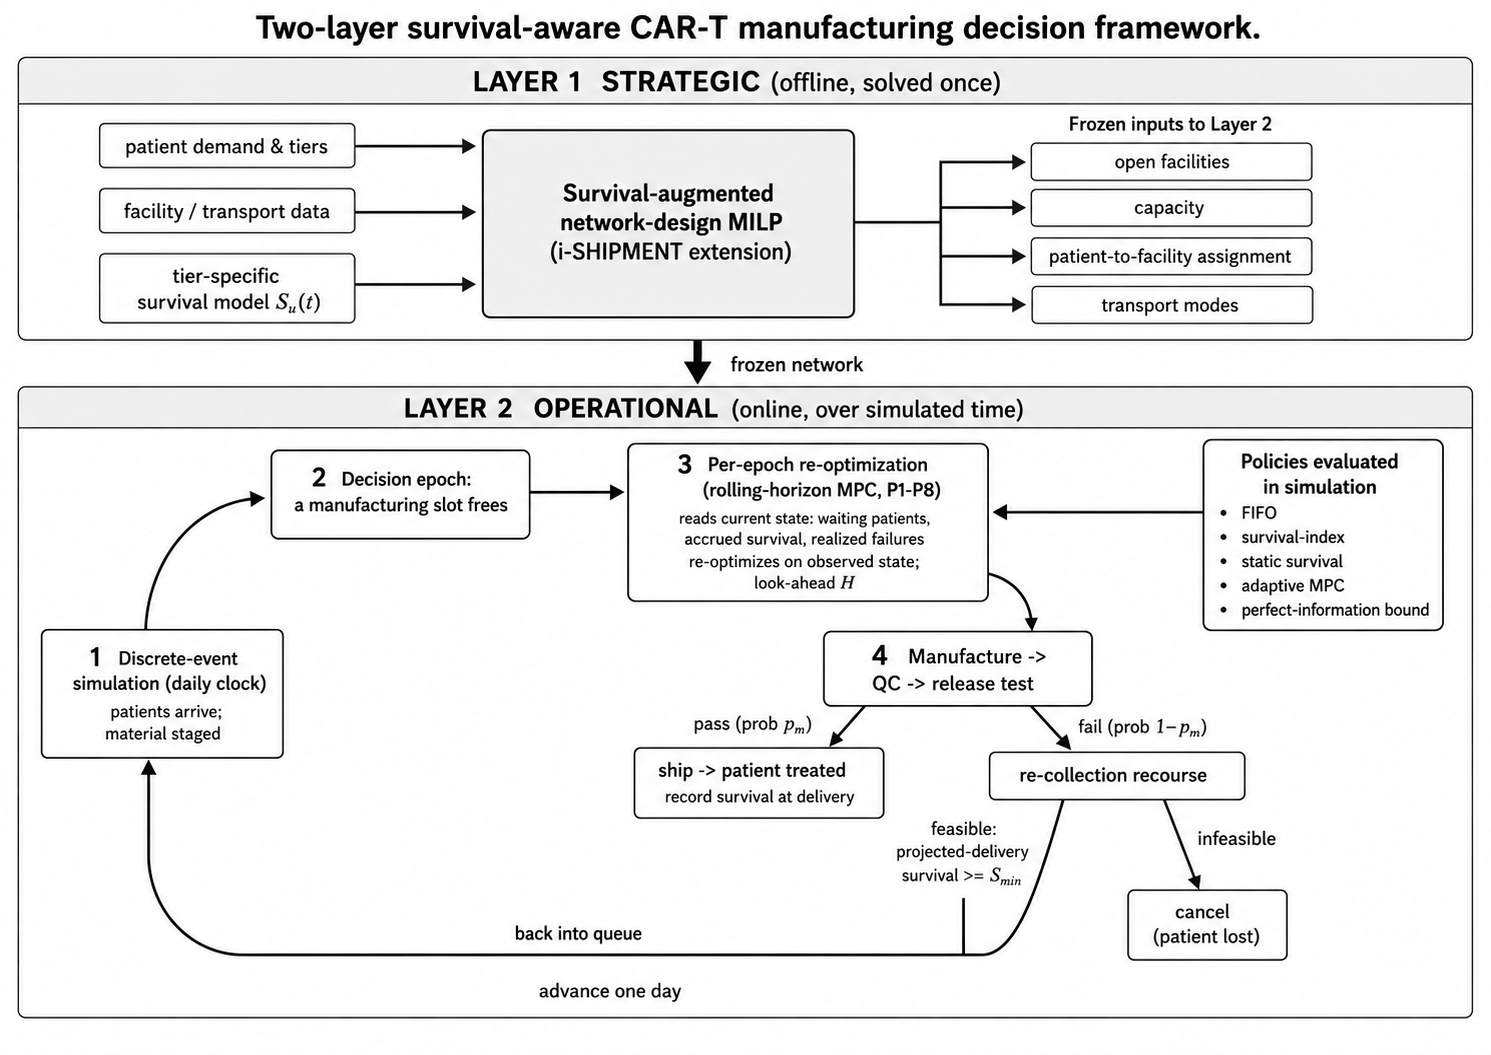
\includegraphics[width=\textwidth]{figures/Framework.png}
  \caption{\textbf{Two-layer survival-aware scheduling framework.} The
  strategic layer is solved once and fixes the network---open facilities,
  capacity, patient--facility assignment and transport modes. The operational
  layer executes on that frozen network: a daily discrete-event simulation
  realises manufacturing yield, and at each epoch at which a slot frees the
  per-epoch problem re-optimises on the observed state over a look-ahead
  window $H$, implementing only the immediate start. A failed batch returns
  its patient to the queue subject to the re-collection gate, or is
  cancelled. All five policies enter at the per-epoch decision point and
  differ only there.}
  \label{fig:framework}
\end{figure}

\subsection{Notation}
\label{sec:notation}

Sets: patients $p \in P$ with risk tier $u(p) \in \{H, M, L\}$; manufacturing
sites $m \in M$; leukapheresis sites $c \in C$; hospitals $h \in H$; transport
modes $j \in J$; periods $t \in T = \{1, \dots, 130\}$; and $\Theta \subset C
\times H$ the set of co-located leukapheresis--hospital pairs.

Parameters retained from the base model: capital and variable facility cost
$\CIM_m$, $\CVM_m$; concurrent capacity $\FCAP_m$; unit transport costs
$\Uone_{cmj}$, $\Uthree_{mhj}$; transport times $\TTone_j$, $\TTthree_j$;
stage durations $\TLS$, $\TMFE$, $\TQC$; per-therapy material and
release-testing costs $\Cmat$, $\CQC$; the arrival incidence $\INC_{pct}$; the
flow bounds $\FMIN$, $\FMAX$; and the maximum turnaround $\ND$.

Parameters introduced here: the tier reference mortality $w_u$ and the induced
hazard $\HR_u$; the survival scale $\eta$ and shape $\gamma$, and sensitivity
$\kappa$; the per-tier value of life $\alphau$; the manufacturing yield
$p_m$; the look-ahead horizon $H$; the re-collection floor $\Smin$; the
maximum number of remakes $\Krem$; and the re-leukapheresis cost $\creleuk$.

Decision variables retained: facility opening $\Eone_m \in \{0,1\}$; link
activation $\Xone_{cm}, \Xtwo_{mh} \in \{0,1\}$; patient routing
$\Yone_{pcmjt}, \Ytwo_{pmhjt} \in \{0,1\}$; the material flow variables
$\LSA$, $\LSR$, $\MSO$, $\OUTC$, $\OUTM$, $\INM$, $\DURV$, $\FTD$, $\INH$; and
the timing variables $\STT_p$, $\CTT_p$, $\TRT_p$. Variables introduced here:
the survival rate $S_p \in [0,1]$; the queue delay $\HOLD_p \ge 0$; the
material arrival $A_{pmt}$; and the survival indicators $\delta_{p,d} \in
\{0,1\}$.

\subsection{Strategic layer: survival-aware network and queue design}
\label{sec:strategic}

\subsubsection{Relationship to the base model}
\label{sec:provenance}

The strategic layer is built on the supply-chain design platform of
Triantafyllou et~al.\ \cite{triantafyllou2022}, and it is worth stating
precisely which components are theirs and which are introduced here.

\emph{Retained without modification.} The network and material-flow structure
is theirs: facility siting and link activation, the patient-routing variables,
the time-indexed material balances that carry each patient's material through
leukapheresis, inbound transport, manufacturing, release testing and outbound
transport, the facility-capacity accounting, the co-location requirement
between collection site and treating hospital, and the cost structure
comprising amortised facility cost, transport cost and per-therapy material and
release-testing cost. In the formulation that follows this is
Equations~\eqref{eq:ctm}--\eqref{eq:atrt}, together with the first three terms
of the objective~\eqref{eq:obj}. The instance data---candidate sites,
capacities, transport times and unit costs---is likewise theirs.

\emph{Introduced in this work.} Four things are new. First, manufacturing start
becomes a decision rather than being identified with material arrival, which
creates the queue and with it the possibility of a deliberate hold,
Equations~\eqref{eq:q1}--\eqref{eq:hold}. Second, patient survival enters the
model explicitly, as the final term of~\eqref{eq:obj} and its exact
linearisation \eqref{eq:surv}--\eqref{eq:lin3}. Third, the maximum-turnaround
constraint is relaxed from the binding timeliness mechanism to a slack outer
bound~\eqref{eq:nd}, for the reason given in \S\ref{sec:linearisation}.
Fourth, the entire operational layer---the per-epoch decision problem, the
execution environment, the policies and the perfect-information
benchmark---has no counterpart in the base model, which is deterministic and
solved once.

\subsubsection{Objective}
\label{sec:objective}

The planner minimises supply-chain cost plus a monetised clinical loss,
\begin{equation}
  \min\; Z \;=\; \sum_{p} \CTM_p \;+\; \sum_{p} \TTC_p
  \;+\; (\Cmat + \CQC)\,|P| \;+\; \sum_{p} \alpha_{u(p)} \bigl(1 - S_p\bigr),
  \label{eq:obj}
\end{equation}
where $\CTM_p$ is the amortised facility cost and $\TTC_p$ the transport cost
of patient $p$,
\begin{align}
  \CTM_p &= \sum_{m} \Eone_m (\CIM_m + \CVM_m)\,|T| / |P|, & &\forall p, \label{eq:ctm}\\
  \TTC_p &= \sum_{c,m,j,t} \Yone_{pcmjt}\, \Uone_{cmj}
            + \sum_{m,h,j,t} \Ytwo_{pmhjt}\, \Uthree_{mhj}, & &\forall p. \label{eq:ttc}
\end{align}

The final term of \eqref{eq:obj} is the contribution of this work. It carries
units of dollars: $\alphau$ is the value of one life lost in risk tier $u$, and
it is the only life-value parameter in the model. There is no dimensionless
triage weight multiplying it. This matters for identification: a formulation
written as a scalar value of life times a priority weight identifies only the
\emph{product} of the two, so the priority weight would be an unfalsifiable
modelling choice dressed as a parameter. Written as $\alphau$, the objective
carries exactly three numbers, each of which is a dollar valuation that can be
quoted, sourced and argued with on its own terms
(\S\ref{sec:calibration}).

We stress that \eqref{eq:obj} contains \textbf{no priority rule, no tier
ordering and no reserved capacity}. Any prioritisation that emerges does so
because $S_p$ falls faster for higher-hazard tiers, which is a property of the
calibration in \S\ref{sec:calibration}, not of the constraint set. The
distinction is testable rather than rhetorical. Under the index
rule~\eqref{eq:index}, patient $i$ is served before patient $j$ whenever
$\alpha_{u(i)} \Delta S_i > \alpha_{u(j)} \Delta S_j$, where $\Delta S$ is the
one-day survival decrement; over the admissible turnaround range the
calibration of \S\ref{sec:calibration} gives $\Delta S_H : \Delta S_M : \Delta
S_L = 7.3 : 2.5 : 1$. High-risk patients are therefore served ahead of low-risk
ones for \emph{any} life-value vector with $\alpha_L / \alpha_H < 7.3$, and
ahead of medium-risk ones for any vector with $\alpha_M / \alpha_H < 2.9$. The
ordering we report is a consequence of the hazard calibration and survives
inversions of $\alphau$ far larger than any defensible valuation would
produce.

\subsubsection{Material balance, capacity and network structure}

Equations~\eqref{eq:bal1}--\eqref{eq:durv} are the time-indexed material
balances of the base model, propagating each patient's material from collection
through leukapheresis, inbound transport, manufacturing, release testing and
outbound transport:
\begin{align}
  \INC_{pct} &= \OUTC_{p,c,t+\TLS}, & &\forall p,c,t, \label{eq:bal1}\\
  \OUTC_{pct} &= \sum_{m,j} \LSR_{pcmjt}, & &\forall p,c,t, \label{eq:bal2}\\
  \LSR_{pcmjt} &= \LSA_{p,c,m,j,t+\TTone_j}, & &\forall p,c,m,j,t, \label{eq:bal3}\\
  A_{pmt} &= \sum_{c,j} \LSA_{pcmjt}, & &\forall p,m,t, \label{eq:arrival}\\
  \INM_{pmt} &= \OUTM_{p,m,t+\TMFE}, & &\forall p,m,t, \label{eq:bal5}\\
  \OUTM_{pmt} &= \sum_{h,j} \MSO_{p,m,h,j,t+\TQC}, & &\forall p,m,t, \label{eq:bal6}\\
  \MSO_{pmhjt} &= \FTD_{p,m,h,j,t+\TTthree_j}, & &\forall p,m,h,j,t, \label{eq:bal7}\\
  \INH_{pht} &= \sum_{m,j} \FTD_{pmhjt}, & &\forall p,h,t, \label{eq:bal8}\\
  \DURV_{pmt} &= \sum_{1<\tau\le t}\bigl(\INM_{p,m,\tau-1} - \OUTM_{p,m,\tau}\bigr)
                 + \OUTM_{pmt}, & &\forall p,m,t. \label{eq:durv}
\end{align}

Equation~\eqref{eq:arrival} is where this model departs from its predecessor.
In the base model the manufacturing start is \emph{identified} with material
arrival: a job begins the day its material reaches the site. Here $A_{pmt}$
records only the arrival, and the start $\INM$ is released as a decision,
governed by the queue \eqref{eq:q1}--\eqref{eq:hold} below.

Concurrent manufacturing at each site is tracked and capped by
\begin{align}
  \RATIO_{mt} &= \sum_{p} \DURV_{pmt} / \FCAP_m, & &\forall m,t, \label{eq:ratio}\\
  \CAPv_{mt} &= \FCAP_m - \sum_{p} \sum_{t-\TMFE \le \tau < t} \INM_{p,m,\tau},
              & &\forall m,t, \label{eq:capdef}\\
  \sum_{p} \INM_{pmt} - \sum_{p} \OUTM_{pmt} &\le \CAPv_{mt}, & &\forall m,t. \label{eq:cap}
\end{align}

The network structure---at most two open facilities, links only to open
facilities, exactly one journey per leg, flow permitted only on activated
journeys, and delivery to the hospital co-located with the collection site---is
carried over unchanged:
\begin{align}
  \sum_{m} \Eone_m &\le 2, \label{eq:con1}\\
  \Xone_{cm} \le \Eone_m,\quad \Xtwo_{mh} &\le \Eone_m, & &\forall c,m,h, \label{eq:con2}\\
  \Yone_{pcmjt} \le \Xone_{cm},\quad \Ytwo_{pmhjt} &\le \Xtwo_{mh},
      & &\forall p,c,m,h,j,t, \label{eq:con3}\\
  \sum_{c,m,j,t} \Yone_{pcmjt} = 1,\quad \sum_{m,h,j,t} \Ytwo_{pmhjt} &= 1,
      & &\forall p, \label{eq:con4}\\
  \sum_{p,h,t} \INH_{pht} &\le |P|, \label{eq:con5}\\
  \Yone_{pcmjt}\,\FMIN \le \LSR_{pcmjt} &\le \Yone_{pcmjt}\,\FMAX,
      & &\forall p,c,m,j,t, \label{eq:con6}\\
  \Ytwo_{pmhjt}\,\FMIN \le \MSO_{pmhjt} &\le \Ytwo_{pmhjt}\,\FMAX,
      & &\forall p,m,h,j,t, \label{eq:con7}\\
  \sum_{m,j,t} \Ytwo_{pmhjt} &= \sum_{t} \INC_{pct},
      & &\forall p,\; \forall (c,h) \in \Theta. \label{eq:con8}
\end{align}

Timing follows
\begin{align}
  \STT_p = \sum_{c,t} t\,\INC_{pct}, \quad
  \CTT_p &= \sum_{h,t} t\,\INH_{pht}, & &\forall p, \label{eq:times}\\
  \TRT_p = \CTT_p - \STT_p, \quad \STT_p &\le \CTT_p, & &\forall p, \label{eq:trt}\\
  \ATRT &= \tfrac{1}{|P|}\sum_{p} \TRT_p, \label{eq:atrt}
\end{align}
where $\TRT_p$ is the turnaround time of patient $p$, measured from collection
to infusion, and $\ATRT$ its cohort average.

\subsubsection{The manufacturing queue}
\label{sec:queue}

Replacing the fixed start with a queue requires four constraints:
\begin{align}
  \sum_{\tau \le t} \INM_{pm\tau} &\le \sum_{\tau \le t} A_{pm\tau},
      & &\forall p,m,t, \label{eq:q1}\\
  \sum_{t} \INM_{pmt} &= \sum_{t} A_{pmt}, & &\forall p,m, \label{eq:q2}\\
  \sum_{p} \DURV_{pmt} &\le \FCAP_m, & &\forall m,t, \label{eq:q3}\\
  \HOLD_p &= \sum_{m,t} t\,\bigl(\INM_{pmt} - A_{pmt}\bigr) \;\ge\; 0,
      & &\forall p. \label{eq:hold}
\end{align}

Constraint~\eqref{eq:q1} forbids a job from starting before its material has
arrived; \eqref{eq:q2} requires each routed material to be started exactly
once; \eqref{eq:q3} caps concurrent manufacturing at each site; and
\eqref{eq:hold} defines the hold, the delay between arrival at the
manufacturing site and the start of manufacturing.

The hold is the \textbf{only new degree of freedom in the model}, and this is
what makes the design identifiable. Capacity~\eqref{eq:q3} forces some
patients to wait; the objective~\eqref{eq:obj} chooses \emph{which} patients
wait. Because the downstream balances \eqref{eq:bal5}--\eqref{eq:bal8} shift
with the chosen start, $\TRT_p$---and hence $S_p$---absorb the wait
automatically, without any additional linking constraint.

\subsubsection{Exact linearisation of survival}
\label{sec:linearisation}

The survival model is
\begin{equation}
  S_p = \exp\Bigl(-\kappa \cdot \HR_{u(p)} \cdot \bigl(\TRT_p / \eta\bigr)^{\gamma}\Bigr),
  \qquad \forall p, \label{eq:surv}
\end{equation}
which is nonlinear in $\TRT_p$. Two features of the problem make an
\emph{exact} linearisation available rather than an approximation. First,
every duration in the network is integral, so $\TRT_p$ is integer-valued.
Second, $\TRT_p$ is bounded below by the fastest feasible route and above by
the turnaround cap,
\[
  \Tmin = \TLS + \min_j \TTone_j + \TMFE + \TQC + \min_j \TTthree_j = 17\ \text{days},
  \qquad \Tmax = \ND = 42\ \text{days},
\]
so $\TRT_p$ is supported on the 26 integers $\{17, \dots, 42\}$. We therefore
introduce binary indicators $\delta_{p,d}$, $d \in \{17,\dots,42\}$, and impose
\begin{align}
  \sum_{d} \delta_{p,d} &= 1, & &\forall p, \label{eq:lin1}\\
  \TRT_p &= \sum_{d} d\,\delta_{p,d}, & &\forall p, \label{eq:lin2}\\
  S_p &= \sum_{d} \sigma_{d,u(p)}\,\delta_{p,d}, & &\forall p, \label{eq:lin3}
\end{align}
with $\sigma_{d,u} = S_u(d)$ precomputed from \eqref{eq:surv}. Because the
support of $\TRT_p$ is exactly the breakpoint set,
\eqref{eq:lin1}--\eqref{eq:lin3} is not a piecewise-linear approximation: it
reproduces \eqref{eq:surv} exactly at every feasible point. This is a
strengthening of the SOS2 $\lambda$-method used in the original model
specification, which the $\delta$-formulation dominates here precisely because
integrality removes the need for interpolation between breakpoints. We report
the implemented formulation rather than the specified one, and note that the
two coincide in value.

Finally,
\begin{equation}
  \TRT_p \le \ND, \qquad \forall p, \label{eq:nd}
\end{equation}
with $\ND$ relaxed from 18 to 42 days. This relaxation is essential and
deserves comment: under $\ND = 18$ the turnaround is pinned to $\{17, 18\}$ and
the survival term of \eqref{eq:obj} has almost no support to act on, so the
model \emph{cannot} express a prioritisation preference. Relaxing $\ND$
converts the deadline from the binding timeliness mechanism into a slack outer
bound, and lets survival---a continuous, tier-specific quantity---drive
timeliness instead. The relaxation does not weaken the clinical requirement; it
relocates it from a constraint to the objective, where it can be traded against
cost at a stated exchange rate.

\subsubsection{Exact reformulation and valid inequalities}

Three reductions make the model tractable at the scales studied without
altering its feasible set or optimal value.

\paragraph{Index reduction.} In every feasible solution the routing variables
collapse: constraints \eqref{eq:con4}, \eqref{eq:con6} and \eqref{eq:con8}
force the single active $\Yone$ of patient $p$ onto its own collection site and
onto the single day $t = t^{0}_{p} + \TLS$, and force the single active
$\Ytwo$ onto the hospital co-located with that site. We therefore replace
$\Yone_{pcmjt}$ by $y1_{pmj}$ and $\Ytwo_{pmhjt}$ by $y2_{pmj}$, eliminating
two index dimensions. Likewise \eqref{eq:ratio}--\eqref{eq:cap} with
\eqref{eq:durv} reduce algebraically to a rolling $\TMFE$-day window on
manufacturing starts, $\sum_{p} \sum_{\tau = t-\TMFE+1}^{t} \INM_{pm\tau} \le
\FCAP_m$. Equivalence of the reduced and full-index formulations is verified
numerically at the 50-patient scale rather than asserted.

\paragraph{Dominance cuts.} Sites $m_4, m_5, m_6$ share the capital cost,
variable cost and capacity of $m_1, m_2, m_3$ respectively but carry weakly
higher transport costs from every collection site. Any solution opening the
dominated site without its counterpart can be relabelled onto the counterpart
at no greater cost and with identical timing, so $\Eone_{m_4} \le \Eone_{m_1}$,
$\Eone_{m_5} \le \Eone_{m_2}$, $\Eone_{m_6} \le \Eone_{m_3}$ are valid and
objective-preserving.

\paragraph{Symmetry breaking.} Patients sharing a collection site, a risk tier
and an arrival day are fully interchangeable---identical costs, arrival
dynamics and survival curves---so requiring their start days to be
non-decreasing removes a symmetry group without cutting off any objective
value.

\paragraph{Aggregate throughput cuts.} Constraint~\eqref{eq:q3} admits at most
$\FCAP_m$ starts in any $\TMFE$ consecutive days. Partitioning the start-window
union into disjoint $\TMFE$-day blocks and applying the argument to every
prefix yields a family of cuts of the form $k \sum_{m} \FCAP_m \Eone_m \ge$
(number of patients whose start window ends by $T$). These are implied by
\eqref{eq:q3} and therefore change neither the feasible set nor the optimum;
they tighten the root relaxation.

\paragraph{Verification.} The three families above are objective-preserving by
construction, but the claim was also checked empirically rather than left as an
argument: every design was re-solved with all three disabled. The optimum was
unchanged in all six cases---exactly in three, and within the $10^{-6}$
optimality tolerance in the other three---while solution times fell by
$2.2\times$ to $9.6\times$ on the cost designs. On the two hardest instances,
$N = 500$ with survival priced, the cuts are the difference between proving
optimality in roughly 130\,s and failing to prove it within a
7200\,s limit. The index reduction is not covered by that test, since
it is the formulation rather than an added inequality; its equivalence is
checked separately against the full-index program, which is only constructible
at small $N$ (491{,}516 columns at twelve patients, against 354 reduced).

\subsubsection{The cost-only comparator}
\label{sec:tiebreak}

Several experiments contrast the survival-aware design against a planner who
minimises cost alone. Setting $\alphau = 0$ does not express that planner, and
using it would make the comparison meaningless. At $\alphau = 0$ the
manufacturing start day $\INM$ carries no objective coefficient---it appears in
neither the facility nor the transport cost---so \emph{every} feasible schedule
is exactly optimal and the resulting survival statistics are whichever member of
that set the solver happened to return. At $N = 200$ we measured 528 pairwise
swaps that improve expected losses at zero objective cost; greedy swapping alone
moves expected losses from 9.880 to 8.521 with the total cost unchanged to the
cent. Six independent solves of the same program returned expected losses
ranging from 9.156 to 9.880, which places a 28\% swing on any benefit measured
against it.

The comparator is therefore solved at a small positive reference value,
$\alpha_{\mathrm{ref}} = \$1$, which renders the objective lexicographic. Cost
still decides every choice that costs money---the survival term can move the
objective by at most about \$30, against a smallest inter-design cost difference
of \$1{,}261, a margin of roughly forty---and survival only ranks schedules of
\emph{equal} cost. The cost-minimising planner thus takes every survival gain
available at no cost, which is what a rational cost minimiser would do, and the
benefit attributed to survival-aware design becomes a lower bound rather than an
artefact of an unlucky tie. At $N = 200$ the tie-break leaves the optimal cost
identical (\$14{,}908{,}756) while expected losses fall from 9.880 to 7.738 and
high-risk mean hold from 9.97 to 1.60 days.

This has a substantive consequence we report rather than conceal: once the
cost-only planner is credited with those free gains, it already serves high-risk
patients first, and the residual benefit of \emph{pricing} survival in the
strategic objective is small (0.49 expected patients at $N = 200$). The gains
that require survival awareness are operational, not architectural.

\subsection{Survival calibration}
\label{sec:calibration}

The survival model is calibrated to a reference six-week mortality rather than
to a hazard ratio, which makes every parameter clinically interpretable and
identifiable from published outcome data.

Let $w_u$ denote the probability that a tier-$u$ patient dies within $\Tref =
42$ days without treatment, so $S_u(42) = 1 - w_u$. Setting $\eta = \Tref$ and
$\kappa = 1$ fixes the scale, and the hazard follows as $\HR_u = -\ln(1 -
w_u)$, which is \emph{derived} rather than assumed. With $w = \{H\!: 0.15,\;
M\!: 0.05,\; L\!: 0.02\}$ this yields $\HR = \{0.163, 0.051, 0.020\}$, a ratio
of roughly $8 : 2.5 : 1$.

We fix the shape $\gamma = 1$, giving a constant baseline hazard and the closed
form
\begin{equation}
  S_u(t) = (1 - w_u)^{t/42}. \label{eq:closedform}
\end{equation}

This is the conservative choice, and the reason matters for the credibility of
the results. Under $\gamma = 1$ a saved day is worth the same at every point in
the patient's wait; any prioritisation benefit the model finds therefore cannot
be an artefact of an accelerating hazard curve that mechanically rewards
serving the sickest first. Values $\gamma = 1.5$ and $2$ are retained only as a
robustness sweep. Survival is monotone for every $\gamma > 0$, so the
qualitative structure is unaffected.

At the minimum turnaround of 17 days the high-risk tier already sits at $S_H =
0.936$ against $S_L = 0.992$---a 5.6-point gap that widens to 13.0 points at 42
days. That gap is the entire room the objective has to work with, and it is
absent from the base model, in which turnaround is pinned to 17--18 days.

\subsubsection{Life-value calibration}

The three numbers $\alphau$ are the only place where a clinical outcome is
converted into dollars, so we state their provenance explicitly. Because the
decision at issue is the allocation of a manufacturing slot---a reimbursement
question---the appropriate yardstick is a health-technology-assessment
threshold rather than a regulatory value of a statistical life. We therefore
take
\[
  \alphau = Q_u \times \lambda,
\]
with $Q_u$ the quality-adjusted life-years a successfully treated tier-$u$
patient gains over salvage therapy and $\lambda$ a willingness-to-pay threshold
per QALY. At $\lambda = \$125{,}000$/QALY, the midpoint of the range in
standard use for US value assessment, and $Q = \{H\!: 12,\, M\!: 8,\, L\!:
4\}$, this gives
\[
  \alpha = \{H\!: \$1.5\text{M},\; M\!: \$1.0\text{M},\; L\!: \$0.5\text{M}\},
\]
which is the vector used throughout. Its level is credible in the sense that
matters for a reimbursement decision: the total valuation per avoided death is
of the same order as the acquisition cost of the therapy itself.

Two caveats belong in the open. First, this is a calibration, not an estimate;
$Q_u$ in particular is not separately identified by the data used here, and a
reader who prefers a different vector can substitute one directly, which is
precisely the advantage of carrying $\alphau$ rather than a product of a value
of life and an unfalsifiable priority weight. Second, the ordering of $\alphau$
is not what drives the results: as shown in \S\ref{sec:objective}, tier
prioritisation under \eqref{eq:index} is unchanged for any $\alphau$ with
$\alpha_L/\alpha_H < 7.3$, so it would survive even a vector that valued
low-risk patients several times above high-risk ones. Experiment~C varies the
level of $\alphau$ by a common multiplier and reports the multiplier at which
the strategic network design itself changes.

\subsection{Operational layer: the per-epoch decision problem}
\label{sec:epoch}

With the strategic layer frozen, a decision epoch occurs whenever a
manufacturing slot frees at an open site. At epoch $t$ the observed state
consists of the ready set $W_t$ of patients whose material is staged at their
assigned site; for each $i \in W_t$, its tier $u(i)$, its accrued wait $a_i$, a
failed-once indicator $\varphi_i$ and its frozen site $m(i)$; and the occupancy
$\busy_m(\tau)$ contributed by in-progress jobs. The only decision is
\[
  x_{i,\tau} \in \{0,1\}: \text{ start patient } i\text{'s manufacturing on day }
  \tau \in [t, t+H] \text{ at } m(i).
\]

Survival is evaluated from the observed state, not from a nominal plan:
\begin{align}
  \elapsed_i(\tau) &= a_i + (\tau - t) + \TMFE + \TQC + \TTthree_{m(i)},
      & &\forall i \in W_t,\ \tau, \label{eq:elapsed}\\
  S_i(\tau) &= \bigl(1 - w_{u(i)}\bigr)^{\elapsed_i(\tau)/42},
      & &\forall i \in W_t,\ \tau. \label{eq:sitau}
\end{align}

Because the survival clock runs continuously from the \emph{first} collection,
$a_i = t - t^{0}_{i}$, and \eqref{eq:elapsed} simplifies to $\elapsed_i(\tau) =
\tau - t^{0}_{i} + \TMFE + \TQC + \TTthree_i$. A remade patient therefore
carries the deterioration of every earlier attempt, which is the property that
makes repeated failure clinically costly rather than merely expensive.

The epoch problem is
\begin{equation}
  \min \sum_{i \in W_t} \alpha_{u(i)} \bigl(1 - \hat{S}_i\bigr), \label{eq:epochobj}
\end{equation}
with effective survival
\begin{equation}
  \hat{S}_i = \sum_{\tau} S_i(\tau)\,x_{i,\tau}
              + d_i\Bigl(1 - \sum_{\tau} x_{i,\tau}\Bigr),
  \qquad d_i = S_i(t+H), \label{eq:shat}
\end{equation}
subject to
\begin{align}
  \sum_{\tau} x_{i,\tau} &\le 1, & &\forall i \in W_t, \label{eq:once}\\
  \sum_{i:\, m(i)=m} \ \sum_{\tau-\TMFE < \tau' \le \tau} x_{i,\tau'}
      &\le \FCAP_m - \busy_m(\tau), & &\forall m,\ \tau \in [t, t+H],
      \label{eq:epochcap}\\
  x_{i,\tau} &= 0, & &\text{for } \tau < t. \label{eq:noearly}
\end{align}

The continuation term $d_i$ in \eqref{eq:shat} is what prevents
\eqref{eq:epochobj} from degenerating into a myopic rule: deferring a patient
past the window is charged at the survival that deferral would cost, so the
model weighs serving a patient now against the damage of not serving them at
all within the horizon. The frozen operational cost $\cop_i$ is inert on a
frozen network---it is a per-patient constant and every started patient is
started exactly once---so it does not enter the argmin and is not monetised
into \eqref{eq:epochobj}. Because \eqref{eq:epochobj} carries no cost term,
only the \emph{shape} of the life-value vector reaches the operational layer:
scaling every $\alphau$ by a common factor rescales the epoch objective without
altering its argmin. The level of $\alphau$ is therefore a strategic parameter
alone, and the operational results reported below are invariant to it.

Two structural properties are worth stating. First, because $m(i)$ is frozen,
the patient set partitions across facilities and \eqref{eq:epochcap} never
couples two of them: the epoch problem \textbf{decomposes exactly by facility},
so solving it per site is solving it globally. Second, only the immediate start
($\tau = t$) is implemented before the simulation advances and the problem is
re-solved; the remainder of the look-ahead plan is discarded, in the standard
receding-horizon manner.

\subsubsection{The interpretable index rule}

In the special case of a single free slot, $H = 0$ and no operational cost,
\eqref{eq:epochobj}--\eqref{eq:noearly} collapse to a closed form:
\begin{equation}
  i^{*} = \arg\max_{i \in W_t}\ \alpha_{u(i)}\bigl[\,S_i(t) - S_i(t+1)\,\bigr].
  \label{eq:index}
\end{equation}

Serve whoever loses the most life value from one further day of
waiting. This is a Whittle-type index: it requires no solver, is inspectable by
a clinician, and is the natural rule to deploy. We evaluate it as a policy in
its own right, and its relationship to the full look-ahead model is an
empirical question we report rather than assume.

One structural property of \eqref{eq:index} under $\gamma = 1$ should be stated,
because it is not obvious and it is not something we designed. Since
\[
  S_u(t) - S_u(t+1) = S_u(t)\,\bigl[1 - (1-w_u)^{1/42}\bigr],
\]
the one-day decrement is \emph{proportional to $S_u(t)$ itself}. Within a tier,
therefore, a patient who has waited longer has a lower survival and hence a
smaller index, so \eqref{eq:index} ranks the least-waited patient first. Between
tiers the rule prioritises the sickest, which is the behaviour this study is
about; within a tier it is anti-FIFO and, in principle, starvation-prone. The
marginal-loss logic is correct on its own terms---a patient already deteriorated
does have less left to lose per additional day---but the consequence is that
low-risk patients absorb long and unequal waits. Where a deployment requires
bounded individual waiting rather than minimum aggregate loss,
\eqref{eq:index} should be paired with a tie-break on $t^{0}_{i}$ or an explicit
waiting-time cap; we report the rule as specified and note the property rather
than silently damping it.

\subsection{Execution environment: discrete-event simulation}
\label{sec:sim}

The simulation advances a daily clock $t = 1, \dots, \Thor = 130$ over the
frozen network. Within each day, events are processed in the following order.

\begin{enumerate}
  \item \textbf{Arrivals.} Patients collected on day $t$ enter the system;
        after $\TLS + \TTone$ days their material is staged and they join $W$.
  \item \textbf{Completions and yield.} A job started on day $s$ holds its slot
        for $\TMFE$ days and frees it on day $s + \TMFE$. $\TQC$ days later it
        is release-tested: it passes with probability $p_m$ and is delivered
        $\TTthree$ days later, at which point the patient is treated and their
        realised survival recorded; it fails with probability $1 - p_m$,
        returning the patient to $W$ with $\varphi_i = 1$ and a larger accrued
        wait.
  \item \textbf{Health update.} Accrued waits advance; because the clock is
        continuous from first collection this is implicit in $t - t^{0}_{i}$.
  \item \textbf{Decision.} For each site with a free slot and ready patients,
        the policy is called and the chosen jobs start.
  \item \textbf{Losses.} A patient leaves the system unserved only through the
        recourse rules of \S\ref{sec:recourse}.
\end{enumerate}

Manufacturing yield is the sole stochastic element. Arrivals are the fixed
instance arrivals and health evolves deterministically given the wait, so
randomness enters at exactly one point and its effect on outcomes is
identifiable. Expected loss is accumulated as the probability sum $\sum_i (1 -
S_i)$ on each replication's realised timeline, with $S = 0$ for a patient never
treated; this is a lower-variance estimator than Bernoulli survival draws and
is exact given the timeline.

\subsubsection{Failure recourse with re-collection}
\label{sec:recourse}

On a manufacturing failure the patient requires a \emph{fresh} leukapheresis.
The recourse is deterministic, consistent with deterministic health evolution.

\paragraph{Feasibility.} Re-collection is admissible if and only if projected
survival at the remake's delivery still clears the floor,
\begin{equation}
  \hat{S}_i(\text{delivery}) =
  \bigl(1 - w_{u(i)}\bigr)^{\bigl[a_i + (\TLS + \TTone) + \mathit{wait}_i
    + \TMFE + \TQC + \TTthree\bigr]/42} \;\ge\; \Smin, \label{eq:gate}
\end{equation}
where $\mathit{wait}_i$ is the days until the next free slot at $m(i)$, read
from the same occupancy $\busy_m(\cdot)$ that \eqref{eq:epochcap} uses. Because
the floor is evaluated on \emph{projected} rather than current survival, sicker
and later patients cross it first, reproducing tier-dependent re-collection
eligibility without introducing a second stochastic primitive.

\paragraph{If feasible,} the remake restarts from collection: $\TLS + \TTone$
days are added before manufacturing can resume, the accrued wait grows
accordingly, and $\creleuk$ is charged. The patient re-enters $W$ as a
$\varphi = 1$, lower-survival competitor.

\paragraph{If infeasible,} or once $\Krem$ remakes are exhausted, the patient is
cancelled and carries the full clinical loss.

There is no calendar-based removal of any kind---no raw-wait eligibility
cutoff. A patient still queueing keeps queueing and is credited with whatever
survival their eventual delivery earns, including deliveries falling beyond the
reporting horizon. \S\ref{sec:limits} documents why this choice is material.

\subsection{Policies compared}
\label{sec:policies}

Five policies are executed on the identical frozen network, with identical
realised failures.

\begin{table}[htbp]
  \centering
  \caption{The five operating policies.}
  \label{tab:policies}
  \begin{tabularx}{\textwidth}{lX}
    \toprule
    Policy & Rule \\
    \midrule
    \texttt{fifo} & Serve in arrival order; no objective. The do-nothing
      reference. \\
    \texttt{survival\_index} & The closed-form index \eqref{eq:index}. \\
    \texttt{static\_survival} & The survival schedule optimised once up
      front---the strategic start order---dispatched greedily and never
      re-solved. Remakes join the back of the order. \\
    \texttt{adaptive\_mpc} & The full per-epoch model
      \eqref{eq:epochobj}--\eqref{eq:noearly}, re-solved at every epoch on the
      observed state. \\
    \texttt{best\_achievable} & A perfect-information benchmark; see
      \S\ref{sec:bound}. \\
    \bottomrule
  \end{tabularx}
\end{table}

The four online policies are strictly non-idling: a free slot is never left
empty while a ready patient waits. This is imposed as an equality on the
immediate starts,
\begin{equation}
  \sum_{i \in W_t} x_{i,t} = \min\bigl(\FCAP_m - \busy_m(t),\ |W_t|\bigr),
  \qquad \forall m, \label{eq:nonidle}
\end{equation}
so that policies differ in \emph{whom} they select and never in \emph{how much}
capacity they use---without \eqref{eq:nonidle}, a policy could appear to reduce
clinical loss simply by withholding capacity.

The design isolates two distinct effects. \texttt{fifo} versus the
survival-aware policies identifies the value of survival awareness.
\texttt{static\_survival} versus \texttt{adaptive\_mpc} identifies the value of
\emph{adaptivity} specifically, since both optimise the same clinical objective
and differ only in whether they re-solve on observed state.

\subsection{The perfect-information benchmark}
\label{sec:bound}

A policy comparison without an attainable floor cannot distinguish a good
policy from an easy instance. We therefore compute, for every replication, the
optimal schedule \emph{given the realised failures}.

Let $f_{i,k} \in \{0,1\}$ indicate that attempt $k$ of patient $i$ fails under
the replication's random draws---known to this model, unknown to every online
policy. Binary variables $x_{i,k,\tau}$ start attempt $k$ of patient $i$ on day
$\tau$. Attempt $k+1$ may be run only if attempt $k$ was run and failed, and no
earlier than that attempt's release plus a re-collection:
\begin{align}
  \sum_{\tau} x_{i,k+1,\tau} &\le \sum_{\tau} x_{i,k,\tau}, & &\forall i,k,
      \label{eq:pi1}\\
  \sum_{\tau} \tau\,x_{i,k+1,\tau} &\ge \sum_{\tau} \tau\,x_{i,k,\tau}
      + \TMFE + \TQC + \TLS + \TTone
      - M\Bigl(1 - \sum_{\tau} x_{i,k+1,\tau}\Bigr), & &\forall i,k.
      \label{eq:pi2}
\end{align}

These are imposed subject to the same rolling-window capacity the simulation
enforces and the same $\Smin$ admissibility~\eqref{eq:gate}. The objective
maximises realised weighted survival, in which only a successful attempt
delivers anything:
\begin{equation}
  \max \sum_{i} \sum_{k:\, f_{i,k}=0} \sum_{\tau}
    \alpha_{u(i)}\, S_{u(i)}\bigl(\tau + \TMFE + \TQC + \TTthree_i - t^{0}_{i}\bigr)
    \, x_{i,k,\tau}. \label{eq:piobj}
\end{equation}

Three points of interpretation are essential. First, the resulting value is a
valid lower bound on the \textbf{monetised clinical loss} $\sum_p
\alpha_{u(p)}(1 - S_p)$---the clinical-loss term of objective~\eqref{eq:obj}---and
\emph{not} on unweighted patient counts; a policy can and does fall below it on
unweighted totals without contradiction, and we report it only against the
quantity it bounds. Second, this benchmark is deliberately exempt from the
non-idling requirement~\eqref{eq:nonidle}: deliberately holding a slot open for
a sicker patient arriving tomorrow is part of what perfect information buys, and
forcing it to be work-conserving would produce something other than a bound.
Third, declining an attempt is itself one of the decisions foresight permits,
since capacity spent on a batch known to fail is capacity denied to another
patient.

The benchmark is executed through the same simulation and accounting code as
every other policy, so that reported costs and metrics are constructed
identically and remain comparable.

\subsection{Experimental design}
\label{sec:design}

\paragraph{Instances.} All experiments use the published network data of the base model---four
collection sites, six candidate manufacturing sites with $\FCAP \in \{4, 31,
10, 4, 31, 10\}$, two transport modes---with cohorts built by tiling the
50-patient base cohort. Tier mix (30/40/30 H/M/L) and the collection-site
distribution are inherited patient by patient, and arrival days are rescaled
into the admissible window so that arrival \emph{density}, and hence
congestion, grows with cohort size. Experiments run at $N = 200$ (primary) and
$N = 100$ (confirmation); the 50-patient cohort is used for schedule-level
illustration.

\paragraph{Replication and variance reduction.} Each configuration is
replicated over 30 yield seeds. The draw governing attempt $k$ of patient $i$
is a deterministic function of (seed, patient, attempt) rather than of call
order, which delivers common random numbers in a strong form: the same batches
fail under every policy, at every offered load, and nested across the
failure-rate sweep. Policy contrasts are therefore paired, and the reported
standard errors are of differences that share their noise.

\paragraph{Design of experiments.} Five experiments address five distinct
questions: the calibration itself (does a day of delay cost tiers
differently?); the prioritisation mechanism (who is served first, and where
does the waiting go?); congestion (when does survival awareness matter?),
varied by compressing or expanding the arrival window on a fixed network so
that offered load moves without confounding the network; the value of life (at
what level of $\alphau$ does the network \emph{design} change?), the only
experiment that
re-solves the strategic layer; the policy benchmark against the bound; and
manufacturing failure rate, swept as a common $(1 - p)$ across all sites so the
abscissa is interpretable.

\paragraph{Reported metrics.} We restrict reporting to five quantities fixed in
advance: expected high-risk patients lost (primary), total expected patients
lost, total cost and cost per therapy, mean hold by tier, and the share of the
\texttt{fifo}-to-\texttt{best\_achievable} gap closed. Both the primary and the
total metric are reported in every experiment, in both directions, so that a
policy which improves one at the expense of the other cannot be presented
selectively.

\subsection{Modelling choices, limitations and reproducibility}
\label{sec:limits}

Several choices bound the interpretation of the results and are stated here
rather than in a concluding caveat.

\paragraph{The re-collection floor is weakly binding.} In \eqref{eq:gate} the
term $\mathit{wait}_i$ is read from in-progress occupancy, which by
construction never looks more than $\TMFE - 1 = 6$ days ahead. The floor $\Smin
= 0.75$ therefore requires an accrued wait exceeding roughly 50 days for the
high-risk tier---and far more for the others---before it can bind. In practice
it binds only for policies whose rigid ordering allows individual patients to
decay substantially. A specification in which $\mathit{wait}_i$ reflected queue
position rather than in-progress occupancy would make the floor active across
all policies; we retain the stated specification and report the consequence
rather than tuning the rule to produce activity.

\paragraph{Removal versus decay.} Because there is no calendar-based removal,
expected loss is dominated by survival decay accumulated while waiting rather
than by patients removed from the system. This is the intended semantics---the
model prices delay, and delay is continuous---but it means ``expected patients
lost'' is an expected-mortality quantity, not a count of censored patients.

\paragraph{Scope of the frozen network.} Assignment and transport mode are
inherited from the strategic solution and are not re-decided per epoch.
Expediting an individual patient by upgrading transport mid-horizon is
therefore outside the policy space, and the reported gains are attributable to
sequencing alone. This understates what a fully flexible operational layer
could achieve and is conservative with respect to our claims.

\paragraph{Horizon spillover.} Deliveries falling beyond the 130-day reporting
horizon are credited with their realised survival rather than discarded or
zeroed. Spillover is below 5\% at the operating point and is reported for every
configuration; at the lowest offered load, where the arrival window is
deliberately stretched beyond the horizon, it is substantially larger and is
reported as such.

\paragraph{Computational implementation.} All programs are implemented in
Pyomo and solved with Gurobi~13.0.3 to a relative MIP gap of $10^{-6}$. Every
strategic and perfect-information program reported here attains that tolerance;
none was terminated by a time limit. The qualitative findings also reproduce
under HiGHS, the open-source solver, though its default tolerance leaves several
designs short of proven optimality, so the reported optima are the Gurobi ones. The per-epoch programs are small---at most a few hundred binary
columns, since the ready queue at a single facility never exceeded 33
patients---which is what makes re-optimisation at every epoch practical rather
than merely conceivable. Every replication records the random seed that
generated it and the strategic solution it was executed against, so each
reported quantity is reproducible from a stated draw.


% ---------------------------------------------------------------------------
% A one-entry bibliography, inlined so that the wrapper compiles with pdflatex
% alone. references.bib carries the same entry for use with BibTeX/biblatex
% when this section is dropped into a host manuscript.
% ---------------------------------------------------------------------------
\begin{thebibliography}{1}
\bibitem{triantafyllou2022}
N.~Triantafyllou et~al.
\newblock A digital platform for the design of patient-centric supply chains.
\newblock \emph{Scientific Reports}, 2022.
\end{thebibliography}

\end{document}
